\PassOptionsToPackage{pdftex,
                        pdfauthor={Pavel Březina},
                        pdftitle={BP - Březina},
                        pdfsubject={Adaptivní přímovazební kompenzace statických sil působících na mechatronický systém}
                        }{hyperref}  
\documentclass[12pt, czech, twoside]{article}
\raggedbottom
\usepackage[czech]{babel}

\usepackage{xstring}

\usepackage[T1]{fontenc} 
\usepackage[utf8]{inputenc}
\usepackage{lmodern}

\usepackage{float}
\usepackage{url}
\usepackage{graphicx}  % balík nutný pro vkládání obrázků
\usepackage{array}
\usepackage{amsmath}
\usepackage{siunitx}
\usepackage{enumitem}
\usepackage{microtype} % lepší zalomení textu
\usepackage{comment}
\usepackage{multirow}
\usepackage{geometry}
\usepackage{subcaption}
\usepackage[dvipsnames]{xcolor}
\usepackage{gensymb}
\usepackage{adjustbox}
\usepackage{placeins}
\usepackage{csvsimple}
\usepackage{mathtools}
\usepackage{etoolbox}
\usepackage{pgffor}
\usepackage{minted}
\usepackage{amssymb}
\usepackage{intcalc}
\usepackage{hyperref}
\hypersetup{
  colorlinks=true,
  linkcolor=RoyalBlue,
  citecolor=Red
  }
\usepackage[all]{hypcap}

\usepackage{pdfpages}
\usepackage{ifthen}

\usepackage{pdflscape}
\usepackage{fancyhdr}% http://ctan.org/pkg/fancyhdr
\usepackage{rotating}
\usepackage[autostyle]{csquotes}
\usepackage{multicol}
\usepackage{bm}
\usepackage{tikz}
\usepackage{attachfile2}

\usepackage{changepage} % check if page is odd or even
\usepackage{layout}
\usepackage[backend=biber,style=authortitle,]{biblatex}
\usepackage{titlesec}
\usepackage[stable]{footmisc} % \footnote in \section
\usepackage{animate}
\usepackage{parskip}

\usepackage{scrextend} % check if page is odd or even but better
\usepackage{afterpage}

\usepackage{csquotes}
\DeclareQuoteAlias{german}{czech}
\MakeOuterQuote{"}
\newenvironment{imagepage}{}{}
\BeforeBeginEnvironment{imagepage}{
  \newpage
  \newgeometry{top=0cm, bottom=0cm}
  \let\tmp\oddsidemargin
\let\oddsidemargin\evensidemargin
\let\evensidemargin\tmp
\reversemarginpar
  \begin{samepage}
    \vspace*{\fill}
    }
    \AfterEndEnvironment{imagepage}{
  \end{samepage}
  \vspace*{\fill}
  \restoregeometry}


\def\imagepageinnermargin{0cm}
\def\imagepageoutermargin{0cm}
\newenvironment{landscapeimagepage}{}{}
\BeforeBeginEnvironment{landscapeimagepage}{
  \newgeometry{top=0cm, bottom=0cm, left=0cm, right=0cm}
  \thispagestyle{empty}
  % \raggedright
  \newgeometry{top=0cm, bottom=0cm, left=\imagepageoutermargin, right=\imagepageinnermargin}
                % \ifthispageodd{\pagecolor{yellow}\afterpage{\nopagecolor}}
                % {\pagecolor{orange}\afterpage{\nopagecolor}}% I'm even
  % \checkoddpage
  % \ifoddpage odd%\newgeometry{top=0cm, bottom=0cm, left=\imagepageoutermargin, right=\imagepageinnermargin}
  % \else%\newgeometry{top=0cm, bottom=0cm, left=\imagepageinnermargin, right=\imagepageoutermargin}
  %   even
  % \fi
  % right je horní strana
  % \newgeometry{top=0cm, bottom=0cm, left=0cm, right=4cm}
  \begin{landscape}
    \thispagestyle{empty}
    % \ifthispageodd{I'm odd}{I'm even}% I'm even
    % \begin{samepage}
    % \vspace*{\fill}
    }
    \AfterEndEnvironment{landscapeimagepage}{
    % \vspace*{\fill}
    % \end{samepage}
  \end{landscape}
  % \raggedbottom
  \restoregeometry
  }

\newenvironment{nomargin}{}{}
\BeforeBeginEnvironment{nomargin}{
  \newgeometry{top=0cm, bottom=0cm, left=0cm, right=0cm}
  \vspace*{\fill}
}
\AfterEndEnvironment{nomargin}{
  \vspace*{\fill}
  \restoregeometry}

\setlength\parindent{0pt}

% https://tex.stackexchange.com/a/102845/255601
\newcommand{\todo}[1]{\textbf{\large{\textcolor{red}{#1}}}}

\newcommand*\centermathcell[1]{\omit\hfil$\displaystyle#1$\hfil\ignorespaces}

\newcommand{\subsubscheme}[2]{
  \begin{landscape}
    \thispagestyle{empty}
    \includepdf[pagecommand={\subsubsection{#1}\label{#1}},
      landscape=true,
      scale=0.95]{#2}
  \end{landscape}
}

\newcommand{\subscheme}[2]{
  \begin{landscape}
    \thispagestyle{empty}
    \includepdf[pagecommand={\subsection{#1}\label{#1}},
      landscape=true,
      scale=0.95]{#2}
  \end{landscape}
}

\newlist{enumerateabc}{enumerate}{1}
\setlist[enumerateabc]{label=\alph*.}

\DeclareMathOperator*{\argmax}{arg~max}
\DeclareMathOperator*{\argmin}{arg~min}
\DeclareMathOperator{\atantwo}{atan2}
\DeclareMathOperator{\diag}{diag}
\DeclareMathOperator{\imresize}{imresize}
\newcommand{\COV}[1]{\operatorname{COV}[#1]}
\newcommand{\E}[1]{\operatorname{E}[#1]}
\newcommand{\VAR}[1]{\operatorname{VAR}[#1]}

\DeclarePairedDelimiter\abs{\lvert}{\rvert}
\DeclarePairedDelimiter\norm{\lVert}{\rVert}

% https://tex.stackexchange.com/a/359261/255601
\let\olditem\item
\newcommand{\todoitem}{\let\item\olditem\color{red}\item\preto\item{\color{black}}}

\newcounter{numFrames}
\newboolean{stop}
\newcommand{\includeanimation}[3]{
  %\setcounter{numFrames}{-1} % fileName_0.pdf ... fileName_?.pdf
  \setcounter{numFrames}{0}
  \setboolean{stop}{false}
  \whiledo{\NOT\boolean{stop}}{
    \stepcounter{numFrames}
    \IfFileExists{#1\thenumFrames.png}{}{
      \addtocounter{numFrames}{-1}
      \setboolean{stop}{true}
    }
  }
  \begin{center}
    \shorthandoff{-}
    \animategraphics[autoplay, controls, loop, #3]{#2}{\detokenize{#1}}{0}{\thenumFrames}
    \shorthandon{-}
  \end{center}
}
\newcommand{\includeanimationframes}[3][]{
  \setcounter{numFrames}{0}
  \setboolean{stop}{false}
  \whiledo{\NOT\boolean{stop}}{
    \stepcounter{numFrames}
    \IfFileExists{#2\thenumFrames.png}{}{
      \addtocounter{numFrames}{-1}
      \setboolean{stop}{true}
    }
  }
  \foreach \n in {0,...,5}{
      % \n
      % \todo{\basiceval{\n*\thenumFrames/5}}
      \includegraphics[#3]{\detokenize{#2}\basiceval{\n*\thenumFrames/5}.png}
      \ifnum\n<3
        #1
      \fi
      \ifnum\intcalcMod{\intcalcInc{\n}}{3}=0
      \else
        \hspace{1cm}
      \fi
    }
}

\def\basiceval#1{\the\numexpr#1\relax}

\renewcommand*{\thefootnote}{[\arabic{footnote}]}

% ================================================================================================================
% https://tex.stackexchange.com/questions/60209/how-to-add-an-extra-level-of-sections-with-headings-below-subsubsection
% https://tex.stackexchange.com/a/60212
\makeatletter
\renewcommand\paragraph{\@startsection{paragraph}{4}{\z@}%
  {-2.5ex\@plus -1ex \@minus -.25ex}%
  {1.25ex \@plus .25ex}%
  {\normalfont\normalsize\bfseries}}
\makeatother
\setcounter{secnumdepth}{4} % how many sectioning levels to assign numbers to
\setcounter{tocdepth}{4}    % how many sectioning levels to show in ToC
% ================================================================================================================
\makeatletter
\newcommand\footnoteref[1]{\protected@xdef\@thefnmark{\ref{#1}}\@footnotemark}
\makeatother

% ================================================================================================================


\usetikzlibrary{shapes,arrows,positioning,calc}

\newboolean{includeAnimations}
\setboolean{includeAnimations}{false}

\newboolean{includeAnimationFrames}
\setboolean{includeAnimationFrames}{true}

\setcounter{tocdepth}{3}    % how many sectioning levels to show in ToC


% \def\imagepageinnermargin{1cm}
% \def\imagepageoutermargin{1cm}

% pro tisk
\def\imagepageinnermargin{2cm}
\def\imagepageoutermargin{0.5cm}


% \newcommand{\getmode}{dark-mode}

% \ifthenelse{\equal{\getmode}{dark-mode}}
%     {% true
%       \pagecolor[rgb]{0,0,0}
%       \color[rgb]{0.95,0.95,0.95}
%     }
\addbibresource{Reference.bib}

\begin{document}
\pagenumbering{gobble}
\begin{center}
    
\includegraphics[height=0.21\textheight]{Img/FAV_logo.pdf}
    
\includegraphics[height=0.21\textheight]{Img/zcu-logo.pdf}
\end{center}
\begin{center}
    \vspace{3cm}
    % \textbf{\LARGE{NURBS spliny pro modelování křivek a povrchů a jejich použití v robotice}}\\
    \LARGE{NURBS spliny pro modelování křivek a povrchů a jejich použití v robotice}
\end{center}
\vfill{}
\noindent
Západočeská Univerzita V Plzni \hfill Pavel Březina\\
Katedra Kybernetiky            \hfill letní semestr\\
PAŘR5                \hfill \today
\thispagestyle{empty}
\newpage
% \null\newpage
% \renewcommand{\labelenumii}{\alph{enumii}.}

\includepdf[pages=-, offset=5mm 0mm]{Img/Zadání BP.pdf}

\vspace*{\fill}
{\begin{center}
    \todo{\Huge{VYNECHAT PŘI TISKU}}
\end{center}}
\vspace*{\fill}
\newpage

\vspace*{\fill}
\section*{Prohlášení}
Předkládám tímto k posouzení a obhajobě bakalářskou práci zpracovanou
na závěr studia na Fakultě aplikovaných věd Západočeské univerzity v Plzni.
\par
Prohlašuji, že jsem bakalářskou práci vypracoval samostatně a výhradně s použitím odborné literatury
a pramenů, jejichž úplný seznam je její součástí.
\par
\vspace{5mm}
V Plzni dne \today \hfill ............................................
% \null\hfill Pavel Březina
\section*{Poděkování}
Rád bych poděkoval Ing. Václavu Helmovi, vedoucímu této bakalářské práce, za řádné vedení, přátelskou komunikaci a věnovaný čas pravidelným konzultacím, které značně pomohly směru vývoje této práce.
\vspace*{\fill}
\newpage
\vspace*{\fill}
\section*{Abstrakt}
Tato práce se zabývá automatickou kompenzací statických sil působících na mechatronický systém pomocí proudové kalibrační tabulky. Konkrétně se v práci prozkoumávají možnosti automatické aktualizace této tabulky pomocí NURBS interpolace a aproximace. Toto zahrnuje interpolaci a aproximaci 2D křivek, 3D křivek, 3D povrchů a 4D nadpovrchů, včetně jejich ukázek na obecných a konkrétních datech týkajících se problému této práce. Výsledkem práce je autonomní aktualizace proudové kalibrační tabulky za využití aproximace 4D nadpovrchu.
\section*{\todo{Klíčová slova}}
\section*{Abstract}
This paper deals with the automatic compensation of static forces acting on a mechatronic system using a current calibration table. Specifically, the work explores the possibilities of automatically updating this table using NURBS interpolation and approximation. This includes the interpolation and approximation of 2D curves, 3D curves, 3D surfaces and 4D hypersurfaces, including their demonstration on general and specific data relevant to the problem of this thesis. The result of this work is an autonomous update of the current calibration table using the 4D hypersurface approximation.
\section*{\todo{Keywords}}

\vspace*{\fill}
\newpage

\thispagestyle{empty}
\tableofcontents
\newpage
\listoffigures
\null\newpage

\pagenumbering{arabic}
\section{Úvod}
V práci je nejprve popsána struktura řídících smyček pohybu lékařského CT manipulátoru Phillips Azurion 7 C20
včetně proudové kalibrační tabulky (CCT). Kalibrační tabulka hraje zásadní roli pro dosažení přesných pohybů jednotlivých kloubů a~zajištění přesného a~konzistentního chování při lékařských zákrocích. Z~důvodu přirozeného opotřebení stroje je však nutná pravidelná rekalibrace, která vede k~nežádoucím odstávkám. Cílem této práce je proto navrhnout řešení, jak minimalizovat potřebu rekurentních manuálních rekalibrací stroje pomocí vhodného algoritmu aktualizace CCT, čímž by se zvýšila přesnost a~spolehlivost manipulátoru a~také snížil počet odstávek stroje.
\par
Tato práce se zabývá řešením pomocí B-spline interpolace/aproximace. Interpolace a~aproximace jsou rozhodujícími technikami pro problém aktualizace CCT, které umožňují vyvodit správné hodnoty v~bodech ležících mimo síť naměřených bodů v~této tabulce.\par
% Navrhované řešení by mohlo výrazně zlepšit proces kalibrace, což by v~konečném důsledku vedlo ke spolehlivějšímu a 
Text je rozdělen na několik hlavních částí:
\begin{enumerate}
    \item \nameref{section: řízený a~říddící systém} --- část zaměřená na řízený a~řídící systém, která obsahuje technické specifikace robota, popis problému a~také zvolený přístup řešení
    \item \nameref{section: NURBS teorie} --- obsáhlá kapitola, ve které je rozebrána veškerá teorie k~NURBS křivkám/povrchům včetně kompletně vlastní implementace v~Matlabu dle knihy \cite{The_NURBS_Book}. Kapitola obsahuje ukázky výsledků jednotlivých algoritmů na obecných datech.
    \item \nameref{section: návrh automatické kalibraci} --- část, ve které jsou vizualizovány výsledky aplikace principů NURBS teorie na reálných datech. Dále v~této kapitole byly také využity techniky z~oblasti zpracování signálů, za účelem nalezení vhodných částí měření, které by se daly využít pro aktualizaci CCT.
\end{enumerate}
Všechny hodnoty poloh a~proudů pro jednotlivé klouby byly v~práci znormovány tak, aby bylo omezeno riziko úniku citlivých dat společnosti Phillips. Jedná se tak o~bezrozměrné veličiny, u~kterých nejsou uvedeny jednotky.
\par
V~případě ukázky animací je zobrazeno pouze 6 snímků pro tištěnou verzi, plná verze animace je obsažena v~příloze či v~digitální verzi dokumentace. Celá tato práce včetně zdrojového kódu je veřejně dostupná online --- \cite{Github}.
% \begin{imagepage}
% https://www.philips.cz/healthcare/product/HCNCVD207/azurion-7-c20-with-flexarm-image-guided-therapy-system
% https://www.philips.de/c-dam/corporate/newscenter/de/press-releases/2019/20190122-azurion-7-c20-mit-flexarm/philips-azurion-7-c20-mit-flexarm-produkt2-un-hs-20190122.download.jpg
\begin{figure}[H]
    \centering
    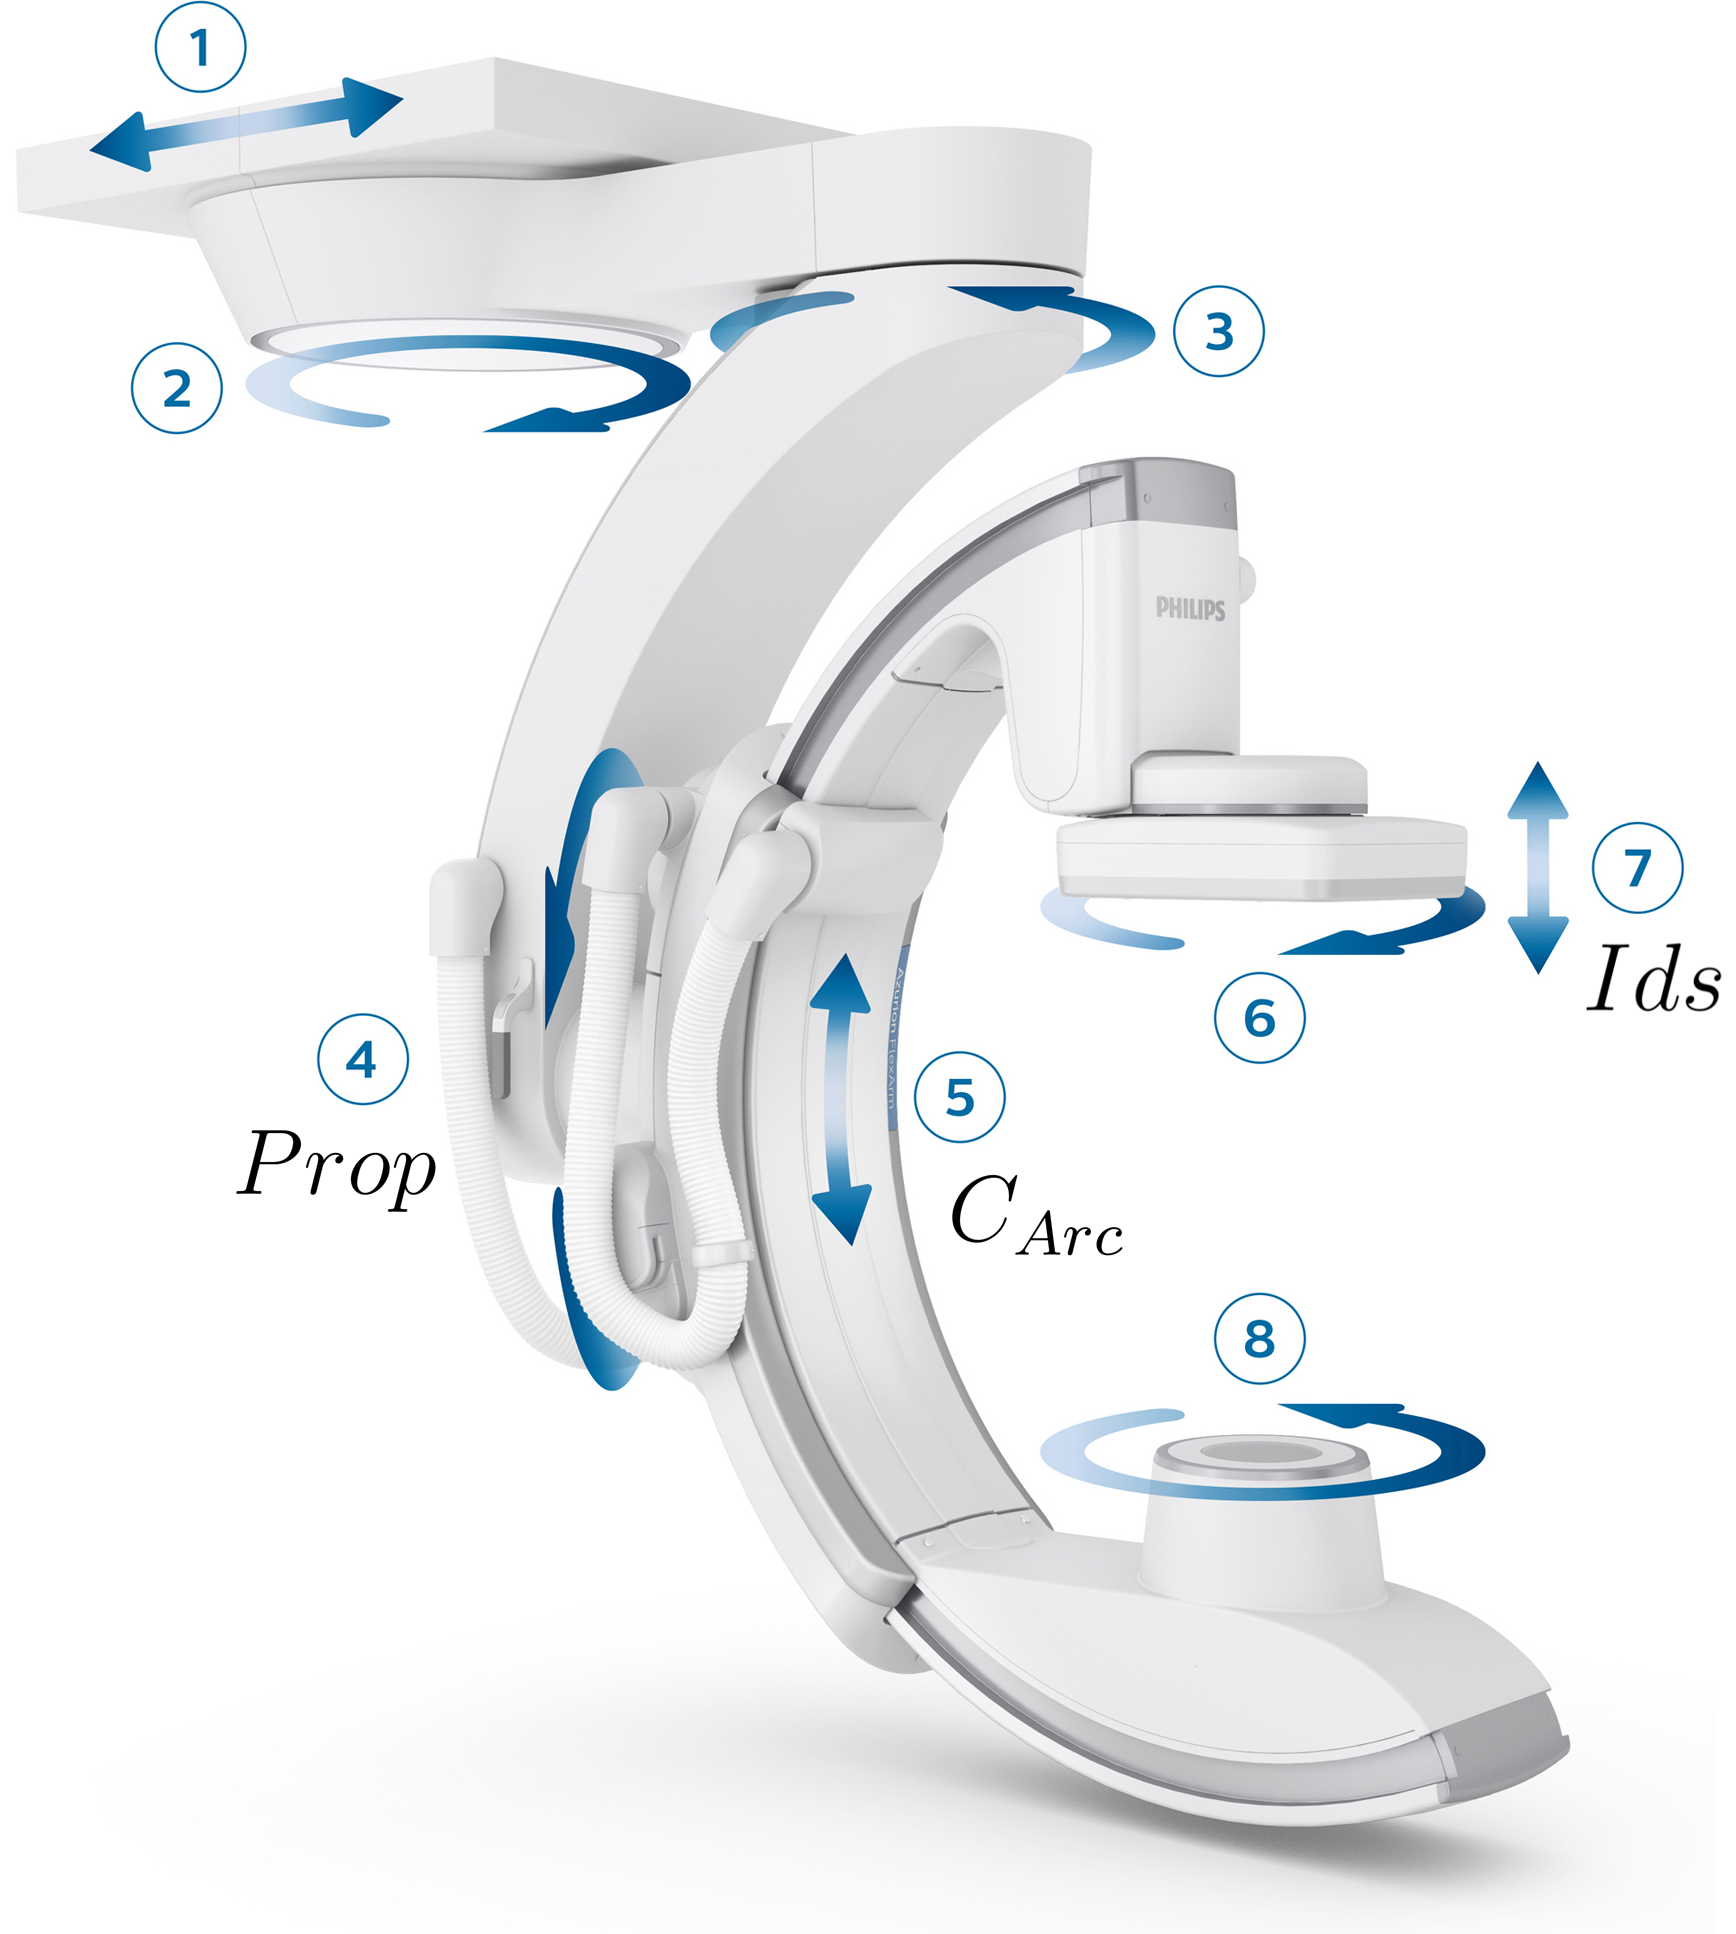
\includegraphics[width=\textwidth]{Img/Azurion 7 C20 with FlexArm modified.png}
    \caption[Výpočetní tomograf s~8 stupni volnosti Phillips Azurion 7 C20]{Výpočetní tomograf s~8 stupni volnosti Phillips Azurion 7 C20 --- \cite{Azurion}}
    \label{fig:Výpočetní tomograf}
\end{figure}
% \end{imagepage}
\section{Řízený a~řídící systém}\label{section: řízený a~říddící systém}
Tato kapitola je zaměřena na popis řízeného systému a~jeho zjednodušeného modelu. Dále je popsána struktura řídícího systému včetně regulační smyčky a~následně je uveden návrh řešení autonomní rekalibrace proudové tabulky.
\subsection{Popis řízeného systému}
Jedná se o~sériový robotický manipulátor s~8 stupni volnosti --- model Phillips Azurion 7 C20. Manipulátor je špičkový lékařský zobrazovací systém určený pro použití v~zákrokové kardiologii a~radiologii\footcite{AzurionPage}. Stroj lze vidět na obrázku č.~\ref{fig:Výpočetní tomograf}.\par
Pro účely této práce jsou klíčové klouby č.~4, 5 a~7, které mají i~své vlastní pojmenování os s~příslušným rozsahem pohybu\footnote{Jak již bylo zmíněno v úvodu, přesné hodnoty byly znormovány z~důvodu důvěryhodnosti dat}:
\begin{itemize}
    \item Kloub č. 5 --- $C_{Arc}\in[0, 1]$
    \item Kloub č. 4 --- $Prop\in[0, 1]$
    \item Kloub č. 7 --- $Ids\in[0, 1]$
\end{itemize}
Pro jednotlivé klouby byla navržena regulační smyčka pohybu na základě fyzikálních parametrů stroje. Tyto parametry se mohou časem měnit, až se nakonec začnou projevovat na průběhu regulace. Toto může být například způsobeno nerovnoměrným opotřebením klíčových dílů zodpovědných za přesný pohyb robota a~nebo například pouhým třením kabelů. Nejen tímto způsobené nepřesnosti lze kompenzovat přímovazební složkou doplněnou o~proudovou kalibrační tabulku.

% Působením času se díly zodpovědné za přesný pohyb robota v~různých místech
% nerovnoměrně opotřebovávají a~to způsobuje nelineární změny fyzikálních
% parametrů, pro které byl daný regulátor pohybu navržen. Tyto nepřesnosti lze
% kompenzovat přímovazební složkou doplněnou o~proudovou kalibrační tabulku.\par

% Pro náš problém budeme uvažovat klouby č. 4, 5 a~7 stroje z~obrázku č. \ref{fig:Výpočetní tomograf}. Klouby mají vlastní pojmenování os a~omezený rozsah pohybu:

\subsection{Zjednodušený model systému}
Nyní vytvoříme zjednodušený 1 DoF model reálného systému (viz obrázek č. \ref{fig:1 DoF schéma robota}), který poslouží pro názornější vizualizaci výsledků dosažených navrženými algoritmy a~jejich snazší otestování a~také porovnání různých přístupů.
Uvažujeme rameno o~délce $l$ a~hmotnosti $m$, které je na jednom konci
ukotvené na hřídeli prostřednictvím rotačního kloubu s~pohonem generující moment síly (točivý moment) $T$. Abychom mohli
nějakým způsobem lépe simulovat změnu fyzikálních parametrů, zavedeme do modelu
také pružnost $k$ a~koeficient tlumení $b$ pohybu ramene. Výsledné schéma je na
obrázku č. \ref{fig:1 DoF schéma robota}.

\begin{figure}[H]
    \centering
    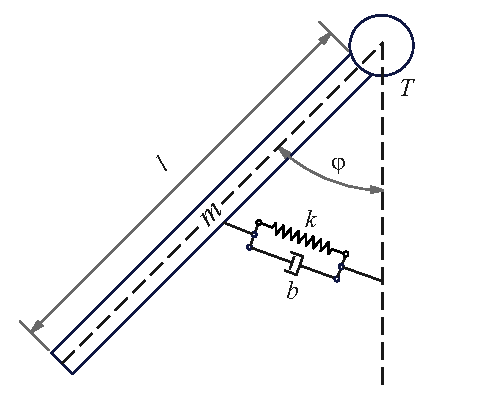
\includegraphics{Img/Drawing.pdf}
    \caption{Schéma zjednodušeného ramene robota}
    \label{fig:1 DoF schéma robota}
\end{figure}
Budeme vycházet z~Newtonovo druhého pohybového zákona pro rotační pohyb --- konkrétně z~rovnice pro moment síly $\bm{M}$, rovnice pro moment hybnosti $\bm{L}$
a jejich vzájemného vztahu:
\begin{align}
    \bm{M} & = \bm{r}\times\bm{F}                             \\
    \bm{L} & = \bm{r}\times\bm{p} = \bm{r}\times m\cdot\bm{v} \\
    \bm{M} & = \frac{d\bm{L}}{dt}
\end{align}
Dosazením parametrů našeho modelu dostáváme:
\begin{align}
    M & = -mgl\cdot\sin(\varphi(t)) -k\cdot\varphi(t) - b \cdot\dot{\varphi}(t) + T(t) \\
    L & =  ml^2\cdot\dot\varphi(t)
\end{align}
Výsledný model je popsán diferenciální rovnicí:
\begin{align}
    \dot{L}                    & =  M                                                                                        \\
    ml^2\cdot\ddot\varphi(t)   & = -mgl\cdot\sin(\varphi(t)) -k\cdot\varphi(t) - b \cdot\dot{\varphi}(t) + T(t)              \\
    \implies \ddot{\varphi}(t) & =  \frac{- mgl\cdot\sin(\varphi(t)) - k\cdot\varphi(t) -b\cdot\dot\varphi(t) + T(t)}{l^2m }
\end{align}
Na tomto modelu můžeme například vykreslit potřebný točivý moment $T$ v~ustáleném stavu ($\ddot{\varphi} = \dot{\varphi} = 0$) pro daný konstantní úhel $\varphi$ na základě různých fyzikálních para\-metrů --- viz obrázek č.~\ref{fig:1 DoF pro různé parametry}. Tímto můžeme simulovat změny fyzických parametrů, které časem probíhají i~na reálném stroji a~také na výsledcích můžeme později odzkoušet interpolační/aproximační algoritmy. V~zásadě se jedná o~proudovou kalibrační tabulku pro náš 1 DoF model, protože točivý moment $T$ je přímo úměrný proudu.
\begin{figure}[H]
    \centering
    \includegraphics{Generated/1 DoF model - změny parametrů.pdf}
    \caption{Potřebný točivý moment motoru pro dosažení úhlu $\varphi$ pro různé parametry 1 DoF modelu}
    \label{fig:1 DoF pro různé parametry}
\end{figure}
\subsection{Struktura řídícího systému}
Kompenzace proudu pohonu pro osu $C_{Arc}$ je závislá na polohách všech tří kloubů
($C_{Arc}$, $Prop$, $Ids$) a~také na směru pohybu\footnote{Kompenzace proudu pohonu pro zbylé osy také pravděpodobně závisí na ostatních osách, nicméně jsou dostupná data pouze pro kompenzační tabulku osy $C_{Arc}$}.

% Pro zatím uvažujeme pouze dvě možné polohy kloubu $Ids$ a~dva možné směry pohybu (dopředný a~zpětný), což nám umožní závislost zaznamenávat pomocí čtyř 2D tabulek. Současná implementace kompenzačních tabulek je postavena právě na tomto rozdělení na 4 tabulky pro každý kloub. 
V současném řídícím algoritmu jsou uvažovány pouze dvě možné polohy kloubu $Ids$ a~dva možné směry pohybu (dopředný a~zpětný), což nám umožní vizualizovat proudovou kalibrační tabulku prostřednictvím čtyř 3D grafů povrchu. Vizualizovaná data z~těchto 4 tabulek pro kloub $C_{Arc}$ lze vidět na obrázcích č. \ref{fig:kompenzace proudu reálná data 1}, \ref{fig:kompenzace proudu reálná data 2},
\ref{fig:kompenzace proudu reálná data 3}, \ref{fig:kompenzace proudu reálná data 4}.

\subsubsection{Schéma regulační smyčky}
K zajištění přesného a~plynulého pohybu regulační smyčka obsahuje 3 hlavní kompenzátory:
\begin{itemize}
    \item $C_{PID}$ --- zpětnovazební PID regulátor, který je zodpovědný za přesné sledování referenční  trajektorie polohy. Regulátor porovnává skutečnou polohu kloubu s požadovanou a na základě jejich rozdílu provádí akční zásahy, aby zajistil co nejpřesnější sledování referenční hodnoty.
    \item $C_{FF}$ --- přímovazební modelově orientovaný regulátor sloužící především ke kompenzaci setrvačnosti a částečně i tření manipulátoru. Tato dopředná vazba se podílí na akční veličině $u$ na základě modelovaných účinků těchto vlivů pro konkrétní stav (např.: poloha, rychlost, zrychlení) a parametry stroje.
    \item $CCT$ --- přímovazební datově orientovaný regulátor v~podobě kompenzační tabulky sloužící ke kompenzaci statické části tření a vnějších momentů způsobených gravitací, vedením kabelů, odporem převodovky a tak podobně. Tato tabulka obsahuje kalibrační hodnoty, které se též podílí na akční veličině $u$ za cílem dosažení co nejplynulejšího pohybu manipulátoru.
\end{itemize}
\pagebreak
Schéma regulační smyčky pro polohu kloubu $C_{Arc}$ vypadá přibližně takto:
\tikzset
{
    block/.style = {draw, fill=white, rectangle, minimum height=2em, minimum width=3em},
    sum/.style n args={4}{draw, fill=white,
            circle, minimum width=6mm, node distance=2cm, path picture={
                    \node at ($(path picture bounding box.south)+(0,0.13)$) {\tiny{#1}};
                    \node at ($(path picture bounding box.west)+(0.13,0)$) {\tiny{#2}}; \node at
                    ($(path picture bounding box.north)+(0,-0.13)$) {\tiny{#3}}; \node at ($(path
                    picture bounding box.east)+(-0.13,0)$) {\tiny{#4}};
                }
        },
    input/.style = {coordinate},
    output/.style= {coordinate},
}

\begin{figure}[H]
    \centering
    \begin{tikzpicture}[auto, node distance=1.5cm,>=latex']
        \shorthandoff{-}
        % \coordinate[] (reference_spacer) {};
        \node[input, label={$r$ \tiny{$[\degree]$}}] (reference) {};
        \node[sum={--}{+}{}{}, right of=reference] (zpetna_vazba) {};

        \node[block, right of=zpetna_vazba, label=below:\tiny{Zpětnovazební reg.}] (zpetnovazebni_reg) {$C_{\text{\tiny{PID}}}$};
        \node[block, above of=zpetnovazebni_reg, label=below:\tiny{Přímovazební reg.}] (primovazebni_reg) {$C_{\text{\tiny{FF}}}$};
        \node[block, above of=primovazebni_reg, label=below:\tiny{Kompenzační tabulka}] (kompenzacni_tab) {$CCT$};
        \node[input, left of=kompenzacni_tab] (other_axis) {};
        \node[input, left of=kompenzacni_tab] (other_other_axis) {};
        \node[sum={}{+}{+}{}, right of=zpetnovazebni_reg] (reg_sum) {};
        \node[block, right of=reg_sum, xshift=1cm, label=below:\tiny{Elektropohon}] (process) {P};
        \node[output, right of=process] (output) {};
        \coordinate [below of=reg_sum,yshift = 0.5cm] (below_reg_sum) {};

        \draw[->] (reference) -- (zpetna_vazba) node [midway, anchor=north] (r) {};
        \node[above of=r] (above_r) {};
        \node[sum={}{+}{+}{}, right of=primovazebni_reg] (right_of_primovazebni_reg) {};
        \node[sum={}{}{}{}, draw=none, right of=kompenzacni_tab] (right_of_kompenzacni_tab) {};
        % \draw[->] (r) |- (kompenzacni_tab);

        \draw[->] (other_axis) node[xshift=-5mm] () {\tiny{$Prop$}}  |- (kompenzacni_tab);
        \begin{scope}[transform canvas={yshift=+3mm}]
            \draw[->] (other_other_axis) node[xshift=-5mm] () {\tiny{$Ids$}} |- (kompenzacni_tab);
        \end{scope}

        \begin{scope}[transform canvas={yshift=-3mm}]
            \draw[->] (above_r) |- (kompenzacni_tab);
        \end{scope}

        \path (kompenzacni_tab) -- node [midway] () {\tiny{$[mA]$}} (right_of_kompenzacni_tab);
        \draw[->] (primovazebni_reg) -- node [midway] () {\tiny{$[A]$}} (right_of_primovazebni_reg);

        \draw[->] (r) |- (primovazebni_reg);
        \draw[->] (r) |- (zpetna_vazba);

        \draw[->] (process) -- node [midway] (y) {$y$ \tiny{$[\degree]$}} (output);
        \draw[->] (reg_sum) -- node [midway] (u) {$u$ \tiny{$[A]$}} (process);
        \draw[->] (zpetnovazebni_reg) -- node [midway] () {\tiny{$[A]$}} (reg_sum);
        \draw[->] (right_of_primovazebni_reg) --  (reg_sum);
        \draw[->] (kompenzacni_tab) -| (right_of_primovazebni_reg);
        \draw[->] (below_reg_sum) -| (zpetna_vazba);
        \draw[-] (y) |- (below_reg_sum);
        \draw[->] (zpetna_vazba) -- (zpetnovazebni_reg);
        \shorthandon{-}
    \end{tikzpicture}
    \caption{Schéma regulační smyčky CT pro jednu osu --- $C_{Arc}$}
\end{figure}
Oba regulátory běžně operují v~řádu ampér, zatímco kompenzační tabulka v~řádu stovek miliampér.
To naznačuje, že tabulka má největší vliv při malých rychlostech (např. při precizních pohybech), kdy výstupy regulátorů jsou v~podobném rozsahu jako výstup proudové kompenzační tabulky.
% Cílem práce je takto uspořádané kompenzační tabulky vhodně automaticky aktualizovat
% na základě naměřených hodnot při běžné činnosti robota.


\begin{landscapeimagepage}
    \begin{figure}[H]
        \centering
        \begin{subfigure}{.5\textheight}
            \centering
            \includegraphics[width=\textwidth]{Generated/Plot kompenzace proudu - reálná data 1.pdf}
            \caption{Vizualizace kompenzační tabulky pro osu $C_{Arc}$ --- dopředný pohyb, $Ids = 0$}
            \label{fig:kompenzace proudu reálná data 1}
        \end{subfigure}
        \vspace{0.5cm}
        \hspace{2.5cm}
        \begin{subfigure}{.5\textheight}
            \centering
            \includegraphics[width=\textwidth]{Generated/Plot kompenzace proudu - reálná data 2.pdf}
            \caption{Vizualizace kompenzační tabulky pro osu $C_{Arc}$ --- dopředný pohyb, $Ids = 1$}
            \label{fig:kompenzace proudu reálná data 2}
        \end{subfigure}
        \vspace{0.5cm}
        \begin{subfigure}{.5\textheight}
            \centering
                    \includegraphics[width=\textwidth]{Generated/Plot kompenzace proudu - reálná data 3.pdf}
                    \caption{Vizualizace kompenzační tabulky pro osu $C_{Arc}$ --- zpětný pohyb, $Ids = 0$}
                    \label{fig:kompenzace proudu reálná data 3}
        \end{subfigure}
        \hspace{2.5cm}
        \begin{subfigure}{.5\textheight}
                \centering
            \includegraphics[width=\textwidth]{Generated/Plot kompenzace proudu - reálná data 4.pdf}
            \caption{Vizualizace kompenzační tabulky pro osu $C_{Arc}$ --- zpětný pohyb, $Ids = 1$}
            \label{fig:kompenzace proudu reálná data 4}
        \end{subfigure}
        \caption{Vizualizace kompenzačních tabulek pro osu $C_{Arc}$}
        \label{fig: Vizualizace kompenzační tabulek pro osu CArc}
    \end{figure}
\end{landscapeimagepage}

% \begin{imagepage}
%     \begin{figure}[H]
%         \centering
%         \includegraphics[width=\textwidth]{Generated/Plot kompenzace proudu - reálná data 1.pdf}
%         \caption{Vizualizace kompenzační tabulky pro osu $x$ - dopředný pohyb, $z = 895$mm}
%         \label{fig:kompenzace proudu reálná data 1}
%     \end{figure}
%     \begin{figure}[H]
%         \centering
%         \includegraphics[width=\textwidth]{Generated/Plot kompenzace proudu - reálná data 2.pdf}
%         \caption{Vizualizace kompenzační tabulky pro osu $x$ - dopředný pohyb, $z = 1170$mm}
%         \label{fig:kompenzace proudu reálná data 2}
%     \end{figure}
% \end{imagepage}

% \begin{imagepage}
%     \begin{figure}[H]
%         \centering
%         \includegraphics[width=\textwidth]{Generated/Plot kompenzace proudu - reálná data 3.pdf}
%         \caption{Vizualizace kompenzační tabulky pro osu $x$ - zpětný pohyb, $z = 895$mm}
%         \label{fig:kompenzace proudu reálná data 3}
%     \end{figure}
%     \begin{figure}[H]
%         \centering
%         \includegraphics[width=\textwidth]{Generated/Plot kompenzace proudu - reálná data 4.pdf}
%         \caption{Vizualizace kompenzační tabulky pro osu $x$ - dopředný pohyb, $z = 1170$mm}
%         \label{fig:kompenzace proudu reálná data 4}
%     \end{figure}
% \end{imagepage}
\subsection{Návrh řešení autonomní rekalibrace proudové tabulky}
Při běžné operaci robota můžeme sledovat polohy a rychlosti jednotlivých kloubů pro které se pohyb vyhlazuje pomocí proudové kalibrační tabulky. Sběrem vhodných bodů pro aktualizaci CCT se zabývá sekce \nameref{section:Analýza záznamu jednoho kloubu}.
\par
Kompenzační proud pohonu pro jeden směr pohybu je momentálně popsán dvěma kalibračními tabulkami (2 polohy kloubu $Ids$), kde každá tabulka popisuje 3D povrch. Nový způsob ukládání těchto závislostí je pomocí 4D NURBS nadpovrchu, což je čtyřrozměrný prostor, který již obsahuje kompletní informaci o kompenzačním proudu pro libovolné polohy všech tří kloubů $C_{Arc}, Prop, Ids$ v rámci jejich stanoveného rozsahu.
\par
Uvažujme tedy kompenzační tabulku popsanou 4D nadpovrchem. Vhodně konstruovaný algoritmus aktivně sleduje pohyby manipulátoru a vyhovující hodnoty kompenzačního proudu uloží pro účely aktualizace CCT. Na základě uložených hodnot můžeme poupravit 4D nadpovrch tak, aby na těchto místech byl kompenzační proud popsán přesněji.
\par
Kroky výsledného algoritmu robota pro jednu relaci by mohly vypadat nějak takto:
\begin{enumerate}
    \item Načtení a vytvoření kalibrační tabulky ve formě NURBS 4D nadpovrchu --- tj. provedení NURBS interpolace \todo{rozvést proč interpolace}
    \item \label{item:průběh práce} V průběhu práce s robotem se za běhu
          \begin{enumerate}
              \item z nadpovrchu vypočítá kompenzační proud na základě aktuálních poloh kloubů $C_{Arc}, Prop, Ids$.
              \item nasbírají vhodné body pro budoucí aktualizaci kompenzační tabulky.
          \end{enumerate}
    \item \label{item:konec relace} Na konci relace na základě nasbíraných bodů proběhne přepočtení a následné uložení kompenzační tabulky  --- tj. provedení NURBS aproximace \todo{rozvést proč aproximace viz článek}
\end{enumerate}
V této práci postupně projdeme všechny tyto zmíněné kroky.
% \section{Linearizace modelu}
\begin{align}
    \bm{x} =
    \begin{bmatrix}
        x_1 \\
        x_2
    \end{bmatrix}
    = \begin{bmatrix}
          \varphi \\
          \dot{\varphi}
      \end{bmatrix}
    \\
    \bm{u} =
    \begin{bmatrix}
        u_1
    \end{bmatrix}
    = \begin{bmatrix}
          T
      \end{bmatrix}
\end{align}
Po zderivování získáme:
\begin{align}
    \bm{\dot{x}} =
    \begin{bmatrix}
        \dot{x}_1 \\
        \dot{x}_2
    \end{bmatrix}
    = \begin{bmatrix}
          \dot{\varphi} \\
          \ddot{\varphi}
      \end{bmatrix}
    =\begin{bmatrix}
         x_2 \\
         \frac{-b\cdot x_2
             - k\cdot x_1
             - g\cdot l \cdot m \cdot\sin(x_1) + u_1
         }{l^2\cdot m}
     \end{bmatrix}
\end{align}
Pokud budeme uvažovat malé úhly $x_1$, můžeme použít aproximaci $\sin(x_1) \approx x_1$:
\begin{align}
    \bm{\dot{x}} =\begin{bmatrix}
                      x_2 \\
                      \frac{-b\cdot x_2
                          - k\cdot x_1
                          - g\cdot l \cdot m \cdot x_1 + u_1
                      }{l^2\cdot m}
                  \end{bmatrix}
\end{align}
Tuto soustavu rovnic již lze snadno zapíšeme pomocí stavového modelu:
\begin{alignat}{2}
          & \bm{A} =
    \begin{bmatrix}
        0                                        & 1                     \\
        \frac{-k -g \cdot l \cdot m}{l^2\cdot m} & \frac{-b}{l^2\cdot m}
    \end{bmatrix}
    \quad &                          &
    \bm{B} =    \begin{bmatrix}
                    0 \\
                    \frac{1}{l^2 \cdot m}
                \end{bmatrix}   \\
          & \bm{C} = \begin{bmatrix}
                         1 & 0 \\
                         0 & 1
                     \end{bmatrix}
    \quad &                          &
    \bm{D} =    \begin{bmatrix}
                    0 \\
                    0
                \end{bmatrix}
\end{alignat}
\section{NURBS teorie}\label{section: NURBS teorie}
Tato kapitola je zaměřena na algoritmy pro práci s NURBS křivkami/povrchy, které jsou ručně implementovány v Matlabu podle knížky \cite{The_NURBS_Book}. V každé podkapitole je uveden odpovídající zdroj z této knížky. Implementace těchto algoritmů je nezbytná pro realizaci autonomní rekalibrace CCT dle návrhu uvedeného v předchozích kapitolách.
% \par
% V kapitole se hojně užívá pojmů ``interpolace'' a ``aproximace'', popřípadě ještě ``extrapolace'', zde je vysvětlení těchto pojmů:
% \begin{itemize}
%     \item Interpolace --- Hledání spojité funkce, jejichž funkční hodnoty odpovídají námi zadaným hodnotám na příslušných souřadnicích. Existuje mnoho interpolačních metod například: lineární interpolace, kosinové interpolace, kubická interpolace a polynomiální interpolace. Zejména polynomiální interpolace není pro naše účely vhodná, protože pro velké množství bodů nabývá vysokého řádu a má tendenci kmitat, toto obzvlášť platí pro ekvidistantně zadané interpolační body.
%     \item Aproximace --- Hledání spojité funkce, která nějakým vhodným způsobem pro danou úlohu nejlépe popisuje aproximační body. Pro naše účely budeme používat NURBS aproximaci založenou na vážené metodě nejmenších čtverců. Tento přístup nám umožní volit stupeň polynomu bázových funkcí, míru redukce bodů (pomocí počtu řídících bodů) a také váhy jednotlivých bodů.
%     \item Extrapolace --- Využití interpolované/aproximované funkce mimo původní rozsah interpolačních/aproximačních bodů. Přesnost extrapolace závisí na charakteru zvolené interpolační/aproximační metody a zdrojových dat. V této práci se extrapolace nevyužívá, protože jí není potřeba, a také proto, že NURBS metodu nelze pro extrapolaci použít.
% \end{itemize}
\subsection[NURBS křivky]{NURBS křivky \footcite[kapitola 3.2]{The_NURBS_Book}}\label{section: NURBS křivky}
Neuniformní racionální B-spline (NURBS) křivku $\bm{C}(u)$\footnote{Jedná se tedy o vektorovou funkci skalární proměnné.} definujeme následovně:
\begin{equation}
    \bm{C}(u) = \sum_{i = 0}^{n} N_{i, p}(u)\bm{P}_i\quad a\le u \le b
\end{equation}
kde
\begin{itemize}
    \item $p$ značí stupeň křivky
    \item $n$ značí počet řídících bodů
    \item $\bm{P}_i$ jsou řídící body, $\dim{\bm{P}_i} \ge 2$
    \item parametry $a$ a $b$ lze znormovat bez ztráty obecnosti --- nejčastěji se udávají hodnoty
          $a = 0$, $b = 1$, které budeme též používat
    \item $N_{i,p}$ jsou B-spline bázové funkce stupně $p$ definované
          na neperiodickém neekvidistantním uzlovém vektoru $\bm{U}$
    \item $u \in \bm{U}$
\end{itemize}
Pro uzlový vektor $\bm{U}$ platí:
\begin{equation}
    \bm{U} = \{\overbrace{\underbrace{a, \ldots, a}_{p + 1}, u_{p + 1}, \ldots, u_{m -p - 1}, \underbrace{b, \ldots, b}_{p + 1}}^{m + 1}\}
\end{equation}
kde $m = n + p + 1$.\par
Bázové funkce lze definovat rekurzivně (výhoda jednoduché implementace):
\begin{align}
    N_{i,0}(u)  & = \begin{cases}
                        1 \quad u_i \le u < u_{i + 1} \\
                        0 \quad jinak
                    \end{cases}                \nonumber         \\
    N_{i, p}(u) & = \frac{u - u_i}{u_{i + p} - u_i}N_{i,p- 1}(u)
    + \frac{u_{i + p + 1} - u}{u_{i + p + 1} - u_{i + 1}}N_{i + 1, p - 1}(u)\label{eq:bázová funkce}
\end{align}
\subsection[NURBS povrchy]{NURBS povrchy\footcite[kapitola 3.4]{The_NURBS_Book}}
Pro sestrojení NURBS povrchu potřebujeme obousměrnou síť řídících bodů $\bm{P}_{i,j}$ a
dva uzlové vektory $\bm{U}$ a $\bm{V}$, poté je možné sestrojit povrch $\bm{S}(u,v)$\footnote{Jedná se tedy o vektorovou funkci dvou skalárních proměnných.}:
\begin{align}
    \bm{S}(u,v) = \sum_{i=0}^{n}\sum_{j=0}^{m}N_{i,p}(u)N_{j,q}(v)\bm{P}_{i,j}
\end{align}
kde
\begin{itemize}
    \item $p$ značí stupeň křivek ve směru $u$
    \item $q$ značí stupeň křivek ve směru $v$
    \item $n$ značí počet řídících bodů ve směru $u$
    \item $m$ značí počet řídících bodů ve směru $v$
    \item $\bm{P}_{i,j}$ je síť řídících bodů, $\dim{\bm{P}_{i,j}} \ge 3$
    \item $u \in \bm{U}$, $v \in \bm{V}$
    \item $a \le u \le b$, $a \le v \le b$ --- stejně jako u \nameref{section: NURBS křivky} budeme uvažovat $a = 0$, $b = 1$ bez ztráty obecnosti
\end{itemize}
Pro uzlové vektory $\bm{U}$ a $\bm{V}$ platí:
\begin{align}
    \bm{U} = \{\overbrace{\underbrace{a, \ldots, a}_{p + 1}, u_{p + 1}, \ldots, u_{r -p - 1}, \underbrace{b, \ldots, b}_{p + 1}}^{r + 1}\}\\
    \bm{V} = \{\overbrace{\underbrace{a, \ldots, a}_{q + 1}, u_{q + 1}, \ldots, u_{s -q - 1}, \underbrace{b, \ldots, b}_{q + 1}}^{s + 1}\}
\end{align}
kde $r = n + p + 1$, $s = m + q + 1$. \par Definice bázových funkcí zůstává stejná --- viz (\ref{eq:bázová funkce}).
\subsection[NURBS interpolace křivky]{NURBS interpolace křivky\footcite[kapitola 9.2.1]{The_NURBS_Book}}\label{section: interpolace křivky}
Mějme množinu $n + 1$ bodů $\{\bm{Q}_k\}$ $k = 0, \ldots, n$, které chceme
interpolovat NURBS křivkou stupně $p$. Pokud každému bodu $\bm{Q}_k$ přiřadíme
parametr $\bar{u}_k$, a vhodně sestrojíme uzlový vektor $\bm{U} = \{u_0, \ldots,
    u_m\}$, můžeme sestavit soustavu lineárních rovnic o rozměru $(n + 1)\times(n +
    1)$:
\begin{equation}
    \bm{Q}_k = \bm{C}(\bar{u}_k) = \sum_{i = 0}^{n}N_{i,p}(\bar{u}_k)\bm{P}_i
\end{equation}
kde řídící body $\bm{P}_i$ tvoří našich $n + 1$ neznámých.\par
Parametr $\bar{u}_k$ lze zvolit více způsoby, z nichž jsou běžné například:
\begin{itemize}
    \item ekvidistantní (equally spaced):
          \begin{alignat}{3}
              \bar{u}_0 & = 0           \quad\quad & \bar{u}_n & =1                 \\
              \bar{u}_k & = \frac{k}{n} \quad\quad & k         & = 1, \ldots, n - 1
          \end{alignat}
          Tato metoda je vhodná pro rovnoměrně rozprostřená data.
    \item délka tětivy (chord length) --- nechť $d$ je celková délka tětivy:
          \begin{equation}
              d = \sum_{k = 1}^{n}\norm{\bm{Q}_k - \bm{Q}_{k - 1}}
          \end{equation}
          potom
          \begin{equation}
              \bar{u}_0 = 0 \quad\quad \bar{u}_n = 1\\
          \end{equation}
          \begin{equation}
              \bar{u}_k = \bar{u}_{k - 1} + \frac{\norm{\bm{Q}_k - \bm{Q}_{k - 1}}}{d}
              \quad\quad k=1,\ldots,n-1
              \label{eq:chord length}
          \end{equation}
          Tato metoda je vhodná pro obecná data.
    \item dostředivá metoda (centripetal method) --- nechť $d$:
          \begin{equation}
              d = \sum_{k = 1}^{n}\sqrt{\norm{\bm{Q}_k - \bm{Q}_{k - 1}}}
          \end{equation}
          potom
          \begin{equation}
              \bar{u}_0 = 0 \quad\quad \bar{u}_n = 1\\
          \end{equation}
          \begin{equation}
              \bar{u}_k = \bar{u}_{k - 1} + \frac{\norm{\bm{Q}_k - \bm{Q}_{k - 1}}}{d}
              \quad\quad k=1,\ldots,n-1
              \label{eq:centripetal method}
          \end{equation}
          Tato metoda je vhodná pro obecná data s náhlými změnami směru.
\end{itemize}
Pro tyto metody je doporučený způsob výpočtu $\bm{U}$ metodou průměrování:
\begin{alignat}{3}
    u_0     & = \ldots = u_p = 0 \quad\quad                      & u_{m-p} & = \ldots = u_m = 1 \nonumber                             \\
    u_{j+p} & =\frac{1}{p}\sum_{i=j}^{j+p-1}\bar{u}_1 \quad\quad & j       & =1,\ldots, n -p    \label{eq:uzlový vektor průměrováním}
\end{alignat}
Nyní můžeme sestavit matici $\bm{N}$ $(n + 1) \times (n + 1)$:
\begin{equation}
    \bm{N} = \begin{bmatrix}
        N_{0,p}(\bar{u}_0)        & \cdots & N_{n+1,p}(\bar{u}_0)       \\
        \vdots                    & \ddots & \vdots                     \\
        N_{0, p}(\bar{u}_{n + 1}) & \cdots & N_{n+1,p}(\bar{u}_{n + 1})
    \end{bmatrix}
\end{equation}
Hledané řídící body $\bm{P}$ již spočteme vyřešením soustavy linárních rovnic:
\begin{align}
    \bm{P} = \bm{N}^{-1}\bm{Q}
\end{align}
Takto zavedená interpolace funguje pro libovolnou dimenzi bodů $\bm{Q}_k$.

\subsubsection{Ukázka 2D interpolace}
Na obrázku č. \ref{fig:Demo interpolace 2D} jsou porovnány zmíněné algoritmy
výpočtu parametru $\bar{u}_k$ pro tyto body:
\begin{equation}
    \bm{Q}_k = \begin{bmatrix}
        \bm{x} & \bm{y}
    \end{bmatrix}
    =\input{Generated/Interpolační body demo 2D.tex}
\end{equation}

\subsubsection{Ukázka 3D interpolace}
Na obrázku č. \ref{fig:Demo interpolace 3D} jsou porovnány zmíněné algoritmy
výpočtu parametru $\bar{u}_k$ pro tyto body:
\begin{equation}
    \bm{Q}_k = \begin{bmatrix}
        \bm{x} & \bm{y} & \bm{z}
    \end{bmatrix}
    =\input{Generated/Interpolační body demo 3D.tex}
\end{equation}

\begin{imagepage}
    \begin{figure}[H]
        \centering
        \includegraphics[width=0.85\textwidth]{Generated/Demo interpolace křivky 2D.pdf}
        \caption{Porovnání algoritmů interpolace ve 2D}
        \label{fig:Demo interpolace 2D}
    \end{figure}
    \begin{figure}[H]
        \centering
        \includegraphics[width=0.85\textwidth]{Generated/Demo interpolace křivky 3D.pdf}
        \caption{Porovnání algoritmů interpolace ve 3D}
        \label{fig:Demo interpolace 3D}
    \end{figure}
\end{imagepage}
% \subsection{Interpolace 4D křivky}
Interpolací 4D křivky je v tomto případě myšlena křivka tvořena 3D body ($x, y,
    z$), které se mění v závislosti na 4. souřadnici $w$. Tudíž nechceme
interpolovat jednu dlouhou 4D křivku (jak jsme dosud dělali v předchozích
případech), ale vlastně několik 3D křivek mezi sebou za využití 4.
souřadnice.\par Tohoto docílíme interpolací samotných bodů příslušných křivek
přes souřadnici $w$, kterou lze vidět na obrázcích č. \ref{fig:Demo 4D
    Interpolace mezi body přes souřadnici w 1}, \ref{fig:Demo 4D Interpolace mezi
    body přes souřadnici w 2}, \ref{fig:Demo 4D Interpolace mezi body přes
    souřadnici w 3}. Dále obrázky č. \ref{fig:Demo 4D Interpolace mezi body přes
    souřadnici w shora 1}, \ref{fig:Demo 4D Interpolace mezi body přes souřadnici w
    shora 2} a \ref{fig:Demo 4D Interpolace mezi body přes souřadnici w shora 3}
značí pohled na přechodové křivky shora, a obrázky č. \ref{fig:Demo 4D
    Interpolace mezi body přes souřadnici w konst x 1}, \ref{fig:Demo 4D
    Interpolace mezi body přes souřadnici w konst x 2} a \ref{fig:Demo 4D
    Interpolace mezi body přes souřadnici w konst x 3} ukazují interpolaci mezi
jedním bodem z každé křivky.

\subsubsection{4D Křivka číslo 1}
Tuto 4D křivku tvoří tři 3D křivky popsané body:
\begin{alignat}{3}
    \bm{Q}_1 & = [\bm{x}, \bm{y}, \bm{z}, \bm{w}] & = & [\bm{x}, \sin(\bm{x}), 10, 0]   \\
    \bm{Q}_2 & = [\bm{x}, \bm{y}, \bm{z}, \bm{w}] & = & [\bm{x}, -\sin(\bm{x}), 0, 100] \\
    \bm{Q}_3 & = [\bm{x}, \bm{y}, \bm{z}, \bm{w}] & = & [\bm{x}, \sin(\bm{x}), 20, 200]
\end{alignat}
kde
\begin{equation}
    \bm{x} = linspace(0, 2\cdot\pi, 25)
\end{equation}
Tyto fáze naší 4D křivky jsou rovnoměrně rozmístěny ve 4. dimenzi, tj.
$\bm{w}$ = $0, 100, 200$ při křivky 1, 2 a 3 respektive. Tímto by přechod mezi křivkami měl
být \todo{rovnoměrný? plynulý? symetrický?}. Ukázka přechodu mezi těmito křivkami je
zobrazena na animaci č. \ref{fig:Demo 4D Interpolace mezi křivkami č. 1}.
\subsubsection{4D Křivka číslo 2}
Tuto 4D křivku tvoří tři 3D křivky popsané body:
\begin{alignat}{3}
    \bm{Q}_1 & = [\bm{x}, \bm{y}, \bm{z}, \bm{w}] & = & [\bm{x}, \sin(\bm{x}), 10, 0]                            \\
    \bm{Q}_2 & = [\bm{x}, \bm{y}, \bm{z}, \bm{w}] & = & [\bm{x}, -\sin(\bm{x}), 0, \text{\textcolor{red}{$50$}}] \\
    \bm{Q}_3 & = [\bm{x}, \bm{y}, \bm{z}, \bm{w}] & = & [\bm{x}, \sin(\bm{x}), 20, 200]
\end{alignat}
kde
\begin{equation}
    \bm{x} = linspace(0, 2\cdot\pi, 25)
\end{equation}
V tomto případě interpolační křivky již nejsou rozmístěny rovnoměrně ve 4. dimenzi,
což v našem případě znamená, že přechod od křivky tvořenou body $\bm{Q}_1$ do křivky
tvořenou $\bm{Q}_2$ je $4\times$ kratší, než přechod od $\bm{Q}_2$ do $\bm{Q}_3$. Toto
je naznačené na obrázcích č.~\ref{fig:Demo 4D Interpolace mezi body přes souřadnici w 2},
\ref{fig:Demo 4D Interpolace mezi body přes souřadnici w shora 2} a
\ref{fig:Demo 4D Interpolace mezi body přes souřadnici w konst x 2},
kde je nepoměr vidět (přestože je zkreslený).
Pořádně lze tento jev vidět až na animaci č. \ref{fig:Demo 4D Interpolace mezi křivkami č. 2},
kde je také celý průběh interpolace.

\subsubsection{4D Křivka číslo 3}
Tuto 4D křivku tvoří tři 3D křivky popsané body:
\begin{alignat}{3}
    \bm{Q}_1 & = [\bm{x}, \bm{y}, \bm{z}, \bm{w}] & = & [\bm{x}, \sin(\bm{x}), 10, 0]                        \\
    \bm{Q}_2 & = [\bm{x}, \bm{y}, \bm{z}, \bm{w}] & = & [\bm{x}, -\sin(\bm{x}), 2.5 + 2.5\cos(2\bm{x}), 100] \\
    \bm{Q}_3 & = [\bm{x}, \bm{y}, \bm{z}, \bm{w}] & = & [\bm{x}, \sin(\bm{x}), 17.5 - 2.5\cos(2\bm{x}), 200]
\end{alignat}
kde
\begin{equation}
    \bm{x} = linspace(0, 2\cdot\pi, 25)
\end{equation}
Zde se pro ukázku interpolované křivky mění i v ose $z$ v závislosti na $x$.
Obrázky k této interpolaci jsou \ref{fig:Demo 4D Interpolace mezi body přes souřadnici w 3},
\ref{fig:Demo 4D Interpolace mezi body přes souřadnici w shora 3},
\ref{fig:Demo 4D Interpolace mezi body přes souřadnici w konst x 3} a
\ref{fig:Demo 4D Interpolace mezi křivkami č. 3}.

\begin{imagepage}
    \begin{figure}[H]
        \centering
        \includegraphics[height=0.4\textheight]{Generated/Interpolace 4D křivky - Interpolace mezi body ve 4. dimenzi č. 1.pdf}
        \caption{Interpolace bodů křivek přes souřadnici $w$ č. 1}
        \label{fig:Demo 4D Interpolace mezi body přes souřadnici w 1}
    \end{figure}
    \begin{figure}[H]
        \centering
        \includegraphics[height=0.4\textheight]{Generated/Interpolace 4D křivky - Interpolace mezi body ve 4. dimenzi (shora) č. 1.pdf}
        \caption{Interpolace bodů křivek přes souřadnici $w$ (pohled shora) č. 1}
        \label{fig:Demo 4D Interpolace mezi body přes souřadnici w shora 1}
    \end{figure}
\end{imagepage}

\begin{imagepage}
    \begin{figure}[H]
        \centering
        \includegraphics[height=0.4\textheight]{Generated/Interpolace 4D křivky - Interpolace mezi body ve 4. dimenzi 1 vlákno č. 1.pdf}
        \caption{Ukázka interpolace pro 1 bod z každé křivky č. 1}
        \label{fig:Demo 4D Interpolace mezi body přes souřadnici w konst x 1}
    \end{figure}
    \ifthenelse{\boolean{includeAnimations}}{
        \begin{figure}[H]
            \centering
            \includeanimation{Generated/4D curve demo 1/frame-}{12.5}{palindrome, height=0.4\textheight}
            \caption{Ukázka průběhu interpolace mezi křivkami přes souřadnici $w$ č. 1}
            \label{fig:Demo 4D Interpolace mezi křivkami č. 1}
        \end{figure}
    }{}
\end{imagepage}
\ifthenelse{\boolean{includeAnimationFrames}}{
    \begin{landscapeimagepage}
        \vspace*{\fill}
        \begin{figure}[H]
            \centering
            \includeanimationframes[\vspace{1cm}]{Generated/4D curve demo 1/frame-}{width=0.28\pdfpageheight}
            \caption{Ukázka průběhu interpolace mezi křivkami přes souřadnici $w$ č. 1}
            \label{fig:Demo 4D Interpolace mezi křivkami č. 1}
        \end{figure}
        \vspace*{\fill}
    \end{landscapeimagepage}}{}
% ======================================
\begin{imagepage}
    \begin{figure}[H]
        \centering
        \includegraphics[height=0.4\textheight]{Generated/Interpolace 4D křivky - Interpolace mezi body ve 4. dimenzi č. 2.pdf}
        \caption{Interpolace bodů křivek přes souřadnici $w$ č. 2}
        \label{fig:Demo 4D Interpolace mezi body přes souřadnici w 2}
    \end{figure}
    \begin{figure}[H]
        \centering
        \includegraphics[height=0.4\textheight]{Generated/Interpolace 4D křivky - Interpolace mezi body ve 4. dimenzi (shora) č. 2.pdf}
        \caption{Interpolace bodů křivek přes souřadnici $w$ (pohled shora) č. 2}
        \label{fig:Demo 4D Interpolace mezi body přes souřadnici w shora 2}
    \end{figure}
\end{imagepage}

\begin{imagepage}
    \begin{figure}[H]
        \centering
        \includegraphics[height=0.4\textheight]{Generated/Interpolace 4D křivky - Interpolace mezi body ve 4. dimenzi 1 vlákno č. 2.pdf}
        \caption{Ukázka interpolace pro 1 bod z každé křivky č. 2}
        \label{fig:Demo 4D Interpolace mezi body přes souřadnici w konst x 2}
    \end{figure}
    \ifthenelse{\boolean{includeAnimations}}{
        \begin{figure}[H]
            \centering
            \ifthenelse{\boolean{includeAnimations}}{\includeanimation{Generated/4D curve demo 2/frame-}{12.5}{palindrome, height=0.4\textheight}}{}
            \caption{Ukázka průběhu interpolace mezi křivkami přes souřadnici $w$ č. 2}
            \label{fig:Demo 4D Interpolace mezi křivkami č. 2}
        \end{figure}
    }{}
\end{imagepage}
\ifthenelse{\boolean{includeAnimationFrames}}{
    \begin{landscapeimagepage}
        \vspace*{\fill}
        \begin{figure}[H]
            \centering
            \includeanimationframes[\vspace{1cm}]{Generated/4D curve demo 2/frame-}{width=0.28\pdfpageheight}
            \caption{Ukázka průběhu interpolace mezi křivkami přes souřadnici $w$ č. 2}
            \label{fig:Demo 4D Interpolace mezi křivkami č. 2}
        \end{figure}
        \vspace*{\fill}
    \end{landscapeimagepage}}{}
% =====================================
\begin{imagepage}
    \begin{figure}[H]
        \centering
        \includegraphics[height=0.4\textheight]{Generated/Interpolace 4D křivky - Interpolace mezi body ve 4. dimenzi č. 3.pdf}
        \caption{Interpolace bodů křivek přes souřadnici $w$ č. 3 \todo{možná jinej pohled}}
        \label{fig:Demo 4D Interpolace mezi body přes souřadnici w 3}
    \end{figure}
    \begin{figure}[H]
        \centering
        \includegraphics[height=0.4\textheight]{Generated/Interpolace 4D křivky - Interpolace mezi body ve 4. dimenzi (shora) č. 3.pdf}
        \caption{Interpolace bodů křivek přes souřadnici $w$ (pohled shora) č. 3}
        \label{fig:Demo 4D Interpolace mezi body přes souřadnici w shora 3}
    \end{figure}
\end{imagepage}

\begin{imagepage}
    \begin{figure}[H]
        \centering
        \includegraphics[height=0.4\textheight]{Generated/Interpolace 4D křivky - Interpolace mezi body ve 4. dimenzi 1 vlákno č. 3.pdf}
        \caption{Ukázka interpolace pro 1 bod z každé křivky č. 3}
        \label{fig:Demo 4D Interpolace mezi body přes souřadnici w konst x 3}
    \end{figure}
    \ifthenelse{\boolean{includeAnimations}}{
        \begin{figure}[H]
            \centering
            \ifthenelse{\boolean{includeAnimations}}{\includeanimation{Generated/4D curve demo 3/frame-}{12.5}{palindrome, height=0.4\textheight}}{}
            \caption{Ukázka průběhu interpolace mezi křivkami přes souřadnici $w$ č. 3 \todo{možná jinej pohled}}
            \label{fig:Demo 4D Interpolace mezi křivkami č. 3}
        \end{figure}
    }{}
\end{imagepage}
\ifthenelse{\boolean{includeAnimationFrames}}{
    \begin{landscapeimagepage}
        \vspace*{\fill}
        \begin{figure}[H]
            \centering
            \includeanimationframes[\vspace{1cm}]{Generated/4D curve demo 3/frame-}{width=0.28\pdfpageheight}
            \caption{Ukázka průběhu interpolace mezi křivkami přes souřadnici $w$ č. 3}
            \label{fig:Demo 4D Interpolace mezi křivkami č. 3}
        \end{figure}
        \vspace*{\fill}
    \end{landscapeimagepage}}{}
\subsection[NURBS interpolace povrchu]{NURBS interpolace povrchu\footcite[kapitola 9.2.5]{The_NURBS_Book}}\label{sec:NURBS interpolace povrchu}
Interpolace povrchu je podobná interpolaci 3D křivky --- máme množinu $(n + 1)
    \times (m + 1)$ bodů $\{\bm{Q}_{k,l}\}$, $k=0,\ldots,n$ a $l=0,\ldots,m$ ležících na mřížce, které
chceme interpolovat NURBS povrchem stupně $p$ a $q$, tzn.:
\begin{equation}
    \bm{Q}_{k,l} = \bm{S}(\bar{u}_k, \bar{v}_l) = \sum_{i=0}^{n}\sum_{j=0}^{m}
    N_{i,p}(\bar{u}_k)N_{j,q}(\bar{v}_l)\bm{P}_{i,j}
\end{equation}
Stejně jako u interpolace křivky musíme vhodně zvolit parametry $\bar{u}_k$ a $\bar{v}_k$
a uzlové vektory $\bm{U}$ a $\bm{V}$.
Užitím běžných metod~(\ref{eq:chord length}) a ($\ref{eq:centripetal method}$) získáme
vektory $\hat{\bar{u}}_k$ a $\hat{\bar{v}}_k$, které musíme poté
zprůměrovat přes všechny hodnoty, tzn:
\begin{alignat}{3}
    \bar{u}_k & = \frac{1}{m + 1}\sum_{j=0}^{m}\hat{\bar{u}}_j \quad\quad & k =0,\ldots,n \\
    \bar{v}_l & = \frac{1}{n + 1}\sum_{j=0}^{n}\hat{\bar{v}}_j\quad\quad  & l =0,\ldots,m
\end{alignat}
Uzlové vektory $\bm{U}$ a $\bm{V}$ spočteme již stejně jako u interpolace křivky,
viz~\ref{eq:uzlový vektor průměrováním}.\par
Oproti křivce, v tomto případě $\bm{P}_{i,j}$ již není matice, ale tenzor. Tento problém můžeme
zjednodušit na interpolaci křivek postupně v obou směrech
zafixováním jedné z proměnných $k$ nebo $l$, tj.:
\begin{equation}
    \bm{Q}_{k,l} =\sum_{i=0}^{n}N_{i,p}(\bar{u}_k)
    \left(\sum_{j=0}^{m}N_{j,q}(\bar{v}_l)\bm{P}_{i,j}\right)
    =\sum_{i=0}^{n}N_{i,p}(\bar{u}_k)\bm{R}_{i,l}
\end{equation}
kde \begin{equation}
    \bm{R}_{i,l} = \sum_{j=0}^{m}N_{j,q}(\bar{v}_l)\bm{P}_{i,j}
\end{equation}
Tato metoda funguje pro libovolné pořadí směru interpolace křivek.
Ukázka interpolace je na obrázcích č. \ref{fig:Demo interpolace povrchu 1}, \ref{fig:Demo interpolace povrchu 2},
\ref{fig:NURBS interpolace kompenzační tabulky proudu č. 1},
\ref{fig:NURBS interpolace kompenzační tabulky proudu č. 2},
\ref{fig:NURBS interpolace kompenzační tabulky proudu č. 3},
\ref{fig:NURBS interpolace kompenzační tabulky proudu č. 4}.

\begin{imagepage}
    \begin{figure}[H]
        \centering
        \includegraphics[width=0.95\textwidth]{Generated/Demo interpolace povrchu 1.pdf}
        \caption{Porovnání algoritmů interpolace ve 2D}
        \label{fig:Demo interpolace povrchu 1}
    \end{figure}
    \begin{figure}[H]
        \centering
        \includegraphics[width=0.95\textwidth]{Generated/Demo interpolace povrchu 2.pdf}
        \caption{Porovnání algoritmů interpolace ve 3D}
        \label{fig:Demo interpolace povrchu 2}
    \end{figure}
\end{imagepage}

\subsubsection[Interpolace 4D nadpovrchu]{Interpolace 4D nadpovrchu\footnote{Téma této sekce již není diskuzí \cite{The_NURBS_Book}, tudíž řešení tohoto problému je již značně postaveno na mých vlastních nápadech realizace.}}\label{section:interpolace 4D povrchu}
Interpolací 4D nadpovrchu je zde myšleno vytvoření vektorové funkce tří skalárních proměnných např.: $\bm{S}(u,v,\psi)$. Uvažujme sadu 3D povrchů definovaných mřížkou bodů o~stejné velikosti $i \times j$. Každý povrch uvažujeme na jiné souřadnici $w$\footnote{Souřadnici $w$ si lze představit jako čas, tím pádem máme sadu 3D povrchů, kde se každý nachází v~jakoby jiném časovém okamžiku.}. Přiřazením souřadnice $w$ každému povrchu získají tuto souřadnici také všechny body těchto povrchů, tj.~každý bod je tvořen souřadnicemi $[x,y,z,w]$. \par
Výpočet má následující kroky:
\begin{enumerate}
    \item Pro konkrétní hodnoty $i, j$ vybereme body $\bm{Q}_{i,j}$ ze všech rovin.
          Pro tuto sadu bodů provedeme interpolaci 4D křivky (viz \nameref{section: interpolace křivky}).
          Tímto získáme $i\times j$ 4D křivek $\bm{C}_{i,j}(u)$.
    \item \label{4D aproximace krok 2} Pro libovolnou hodnotu $w$, $w_{min} \le w \le w_{max}$ najdeme body $\hat{\bm{Q}}_{i,j}$ na všech křivkách $\bm{C}_{i,j}(u)$ takové, že 4. souřadnice bodů $\hat{\bm{Q}}_{i,j}$ odpovídá zvolené hodnotě~$w$\footnote{Tento výpočet, pokud vím, nelze provést analyticky, existují pouze heuristické metody. Proto pro nalezení vhodné hodnoty s~nějakou stanovenou přesností jsem použil metodu půlení intervalu, jelikož horní mez $w_{max}$ a~dolní mez $w_{min}$ jsou známy.}.
    \item \label{4D aproximace krok 3} Předchozím krokem jsme získali mřížku bodů $\hat{\bm{Q}}_{i,j}$ pro konkrétní hodnotu $w$.
          Mřížku stačí proložit povrchem pomocí \nameref{sec:NURBS interpolace povrchu} a~již dostáváme nadpovrch pro danou hodnotu souřadnice $w$\footnote{Opakováním kroků \ref{4D aproximace krok 2} a \ref{4D aproximace krok 3} lze vypočítat zbylé potřebné povrchy s~libovolným rozlišením souřadnice~$w$.}.
\end{enumerate}
Nadpovrch lze vizualizovat například pomocí animace jako průchod mezi klasickými povrchy prostřednictvím zbývající proměnné $w$.
Tento algoritmus je například vhodný v~případě, že bychom chtěli vyplnit ``prázdný'' prostor souřadnice $Ids$ mezi tabulkami \ref{fig:kompenzace proudu reálná data 1} a \ref{fig:kompenzace proudu reálná data 2}.\par
Vizualizaci 4D povrchu, který je tvořen třemi 3D povrchy:
\begin{alignat}{3}
    \bm{Q}_{i,j}(1) & = [\bm{X}, \bm{Y}, \bm{Z}, \bm{W}] & = & [\bm{X}, \bm{Y}, \cos(\bm{X}) + \bm{Y}, 10]                   \\
    \bm{Q}_{i,j}(2) & = [\bm{X}, \bm{Y}, \bm{Z}, \bm{W}] & = & [\bm{X}, \bm{Y}, \cos(\bm{Y}) + \bm{X}, 20]                   \\
    \bm{Q}_{i,j}(3) & = [\bm{X}, \bm{Y}, \bm{Z}, \bm{W}] & = & [\bm{X}, \bm{Y}, \cos(2\cdot\bm{Y}) + \cos(2\cdot\bm{X}), 30]
\end{alignat}
lze vidět na animaci na obrázku č.~\ref{fig:Demo 4D Interpolace mezi povrchy č. 1}.
\ifthenelse{\boolean{includeAnimations}}{
    \begin{landscapeimagepage}
        \begin{figure}[H]
            \centering
            \includegraphics[width=0.33\pdfpagewidth]{Generated/Interpolace 4d povrchu část 1 č. 1.pdf}\hspace{0.5cm}
            \includegraphics[width=0.33\pdfpagewidth]{Generated/Interpolace 4d povrchu část 2 č. 1.pdf}\hspace{0.5cm}
            \includegraphics[width=0.33\pdfpagewidth]{Generated/Interpolace 4d povrchu část 3 č. 1.pdf}
            \caption{Interpolační povrchy pro 4D interpolaci č. 1}
        \end{figure}
        \vfill
        \begin{figure}[H]
            \centering
            \includeanimation{Generated/4D surface demo 1/frame-}{12.5}{palindrome, height=0.5\textheight}
            % \includeanimation{Generated/4D surface demo 1/frame-}{12.5}{palindrome, height=0.5\textheight}
            \caption{Ukázka průběhu interpolace mezi povrchy přes souřadnici $w$ č. 1}
            \label{fig:Demo 4D Interpolace mezi povrchy č. 1}
        \end{figure}
    \end{landscapeimagepage}
}{}
\ifthenelse{\boolean{includeAnimationFrames}}{
    \begin{landscapeimagepage}
        \begin{figure}[H]
            \centering
            \includegraphics[width=0.33\pdfpagewidth]{Generated/Interpolace 4d povrchu část 1 č. 1.pdf}\hspace{0.5cm}
            \includegraphics[width=0.33\pdfpagewidth]{Generated/Interpolace 4d povrchu část 2 č. 1.pdf}\hspace{0.5cm}
            \includegraphics[width=0.33\pdfpagewidth]{Generated/Interpolace 4d povrchu část 3 č. 1.pdf}
            \caption{Interpolační povrchy pro 4D interpolaci č. 1}
        \end{figure}
        \vfill
        \begin{figure}[H]
            \centering
            \includeanimationframes{Generated/4D surface demo 1/frame-}{height=0.235\pdfpagewidth}
            % \includeanimation{Generated/4D surface demo 1/frame-}{12.5}{palindrome, height=0.5\textheight}
            \caption{Ukázka průběhu interpolace mezi povrchy přes souřadnici $w$ č. 1}
            \label{fig:Demo 4D Interpolace mezi povrchy č. 1}
        \end{figure}
    \end{landscapeimagepage}
}{}


\subsection{NURBS aproximace křivky\label{sec:NURBS aproximace křivky}}
Mějme množinu $m + 1$ bodů $\bm{Q_k}$ ${k = 0, \ldots, m}$ a hledáme
křivku stupně $p$ ve tvaru:
\begin{equation}
    \bm{C}(u) = \sum_{i = 0}^{n}N_{i,p}(u)\bm{P}_i\quad u\in[0,1], \quad\quad n \ge p \ge 1
\end{equation}
pro kterou platí:
\begin{itemize}
    \item krajní body interpoluje, tj.: $\bm{Q}_0 = \bm{C}(0)$, $\bm{Q}_m = \bm{C}(1)$
    \item zbytek bodů aproximuje váženou metodou nejmenších čtverců:
          \begin{align}
              \bm{P} = (\bm{N}^T \bm{W} \bm{N})^{-1}\bm{R}
          \end{align}
          kde
          \begin{itemize}
              \item $\bm{N}$ je matice $(m - 1) \times (n - 1)$:
                    \begin{equation}
                        \bm{N} = \begin{bmatrix}
                            N_{1,p}(\bar{u}_1)        & \cdots & N_{n-1,p}(\bar{u}_1)     \\
                            \vdots                    & \ddots & \vdots                   \\
                            N_{1, p}(\bar{u}_{m - 1}) & \cdots & N_{n-1,p}(\bar{u}_{m-1})
                        \end{bmatrix}
                    \end{equation}
              \item $\bm{R}$ je matice $(n - 1)\times(\dim\bm{Q})$:
                    \begin{equation}
                        \bm{R} =
                        \begin{bmatrix}
                            N_{1,p}(\bar{u}_1)\omega_1\bm{R}_1 + \cdots + N_{1, p}(\bar{u}_{m - 1})\omega_{m-1}\bm{R}_{m - 1}     \\
                            \vdots                                                                                                \\
                            N_{n-1,p}(\bar{u}_1)\omega_1\bm{R}_1 + \cdots + N_{n-1, p}(\bar{u}_{m - 1})\omega_{m-1}\bm{R}_{m - 1} \\
                        \end{bmatrix} \\
                    \end{equation}
                    kde
                    \begin{equation}
                        \bm{R}_k  = \bm{Q}_k - N_{0, p}(\bar{u}_k)\bm{Q}_0 - N_{n,p}(\bar{u}_k)\bm{Q}_m \quad\quad k = 1, \ldots, m -1
                    \end{equation}
              \item $\bm{W}$ je diagonální matice $(m - 1) \times (m - 1)$\footnote{Váhy
                        krajních bodů nehrají roli, protože tyto body jsou interpolovány}
                    s váhami jednotlivých bodů:
                    \begin{equation}
                        \bm{W}  = \begin{bmatrix}
                            \omega_1 & 0        & \cdots & 0            \\
                            0        & \omega_2 & \cdots & 0            \\
                            \vdots   & \vdots   & \ddots & \vdots       \\
                            0        & 0        & \cdots & \omega_{m-1}
                        \end{bmatrix}
                    \end{equation}
              \item $\bm{P}$ je matice hledaných řídících bodů $(n + 1)\times(\dim\bm{Q})$

          \end{itemize}
\end{itemize}
Opět musíme vhodně zvolit parametry $\bar{u}_k$ a uzlový vektor $\bm{U}$. Parametr $\bar{u}$
můžeme vypočítat pomocí předpisu \ref{eq:chord length}.
\par Prvky uzlového vektoru poté vypočteme následovně:
\begin{equation}
    d = \frac{m + 1}{n - p + 1}
\end{equation}
\begin{alignat}{3}
    i         & = \lfloor j \cdot d \rfloor                                 & \quad\quad \alpha    & = j \cdot d - i              \\
    u_{p + j} & = (1 - \alpha)\cdot\bar{u}_{i - 1} + \alpha \cdot \bar{u}_i & \quad\quad j         & = 1, \ldots, n - p           \\
    u_0       & = \ldots = u_p = 0 \quad\quad                               & \quad\quad u_{n + 1} & = \ldots = u_{n + p + 1} = 1
\end{alignat}
Výsledky tohoto algoritmu lze vidět na obrázcích č.~\ref{fig:Demo aproximace křivky 5}, \ref{fig:Demo aproximace pro
    různé váhy 1}, \ref{fig:Demo aproximace pro různé váhy 2}, \ref{fig:Demo
    aproximace pro různé váhy 3}.+
\begin{imagepage}
    \begin{figure}[H]
        \centering
        \includegraphics[width=0.85\textwidth]{Generated/Demo aproximace křivky 5.pdf}
        \caption{Aproximace křivky metodou nejmenších čtverců pro různé parametry}
        \label{fig:Demo aproximace křivky 5}
    \end{figure}
    \begin{figure}[H]
        \centering
        \includegraphics[width=0.85\textwidth]{Generated/Ukázka aproximace pro různé váhy bodů 1.pdf}
        \caption{Aproximace křivky metodou nejmenších čtverců pro různé váhy bodů}
        \label{fig:Demo aproximace pro různé váhy 1}
    \end{figure}
\end{imagepage}

\begin{imagepage}
    \begin{figure}[H]
        \centering
        \includegraphics[width=0.85\textwidth]{Generated/Ukázka aproximace pro různé váhy bodů 2.pdf}
        \caption{Aproximace křivky metodou nejmenších čtverců pro různé váhy bodů}
        \label{fig:Demo aproximace pro různé váhy 2}
    \end{figure}
    \begin{figure}[H]
        \centering
        \includegraphics[width=0.85\textwidth]{Generated/Ukázka aproximace pro různé váhy bodů 3.pdf}
        \caption{Aproximace křivky metodou nejmenších čtverců pro různé váhy bodů}
        \label{fig:Demo aproximace pro různé váhy 3}
    \end{figure}
\end{imagepage}
\subsubsection{Cílená NURBS aproximace křivky}
Pro naše využití bychom v mnoha případech chtěli aproximovat pouze část křivky
a zbytek interpolovat, proto zavedeme tzv. cílenou aproximaci. Mějme množinu $m
    + 1$ bodů $\bm{Q}_k$ $k = 0, \ldots, m$ a aproximační interval $\bm{I}_{ap}
    \subset \bm{Q}_k$ o délce $l$.\par Na tomto intervalu $\bm{I}_{ap}$ provedeme
aproximaci ze sekce \ref{sec:NURBS aproximace křivky} s $n$ řídícími body, $n
    \le l - 2$. Tímto získáme křivku, ze které vybereme několik vhodných (např.
$2n$ ekvidistantních) bodů~$\bm{Q}_{ap}$. Interval $\bm{I}_{ap}$ v $\bm{Q}_k$
nahradíme body $\bm{Q}_{ap}$ a provedeme interpolaci. \par Tímto se i vhodně
vyhneme problému, který u aproximace nastává v případě $n \sim l$, protože si
lze snadno ohlídat počet řídících bodů $n$ k počtu aproximačních bodů $l$.

\subsection{NURBS aproximace povrchu\label{section:aproximace povrchu}}
Stejně jako u interpolace počítáme s množinou $(r + 1)\times(s + 1)$ bodů
$\bm{Q}_{k,l}$, $k=0,\ldots, r$ a $l = 0, \ldots, s$ ležících v mřížce, které chceme aproximovat
pomocí vážené metody nejmenších čtverců NURBS povrchem stupně $p$ a $q$ ve
tvaru:
\begin{align}
    S(\bar{u}_k, \bar{v}_l) = \sum_{i=0}^{r}\sum_{j=0}^{s}N_{i,p}(\bar{u}_k)N_{j,q}(\bar{v}_l)\bm{P}_{i,j}
\end{align}
Tento algoritmus interpoluje všechny rohové body a zbytek aproximuje, tj. aproximovaná plocha je tvořena body:
\begin{align}
    \begin{matrix}
        \bm{Q}_{0, 0}         & \hat{\bm{Q}}_{0, 1} & \cdots & \hat{\bm{Q}}_{0, s-1}   & \bm{Q}_{0, s}         \\
        \hat{\bm{Q}}_{1, 0}   & \ddots              &        &                         & \hat{\bm{Q}}_{1, s}   \\
        \vdots                &                     & \ddots &                         & \vdots                \\
        \hat{\bm{Q}}_{r-1, 0} &                     &        & \ddots                  & \hat{\bm{Q}}_{r-1, s} \\
        \bm{Q}_{r, 0}         & \hat{\bm{Q}}_{r, 1} & \cdots & \hat{\bm{Q}}_{r-1, s-1} & \bm{Q}_{r,s}          \\
    \end{matrix}
\end{align}
kde $\hat{\bm{Q}}_{i,j}$ je aproximovaný body $\bm{Q}_{i,j}$.\par
Stejně jako u interpolace povrchu budeme nejprve aproximovat křivky
v jednom směru a poté ve druhém. Parametry $\bar{u}_k$ a $\bar{v}_l$ a uzlové
vektory $\bm{U}$ a $\bm{V}$ získáme stejně jako
u interpolace povrchu~-~viz~\ref{sec:NURBS interpolace povrchu}.
Nejprve aproximujeme body ve směru $u$, tím získáme tenzor řídících
bodů aproximačních křivek $\bm{T}$ o rozměrech $(n + 1) \times (s + 1) \times (\dim{\bm{Q}})$:
\begin{alignat}{3}
    \bm{T}_{0, i}              & = \bm{Q}_{0, i}                                   & \quad i = 0, \ldots, s \\
    \bm{T}_{n, i}              & = \bm{Q}_{r, i}                                   & \quad i = 0, \ldots, s \\
    \bm{T}_{1 \ldots n - 1, i} & = (\bm{N}_u^T\bm{W}_u(i)\bm{N}_u)^{-1}\bm{R}_u(i) & \quad i = 0, \ldots, s
\end{alignat}
kde:
\begin{itemize}
    \item $\bm{N}_u$ je matice $(r - 1) \times (n - 1)$:
          \begin{align}
              \bm{N}_u = \begin{bmatrix}
                             N_{1,p}(\bar{u}_1)        & \cdots & N_{n-1,p}(\bar{u}_1)     \\
                             \vdots                    & \ddots & \vdots                   \\
                             N_{1, p}(\bar{u}_{r - 1}) & \cdots & N_{n-1,p}(\bar{u}_{r-1})
                         \end{bmatrix}
          \end{align}
    \item $\bm{W}_u(i)$ je matice $(r + 1)\times(s + 1)$ obsahující váhy
          bodů $\bm{Q}_{0\ldots r, 0 \ldots,s}$:
          \begin{align}
              \bm{W}_u(i)
              = \begin{bmatrix}
                    \omega^u_0(i) & 0             & \cdots & 0               \\
                    0             & \omega^u_1(i) & \cdots & 0               \\
                    \vdots        & \vdots        & \ddots & \vdots          \\
                    0             & 0             & \cdots & \omega^u_{r}(i)
                \end{bmatrix}
              = \diag(\bm{W}_{0\ldots r, i})
          \end{align}
          kde matice $\bm{W}$ obsahuje váhy jednotlivých bodů, tj.
          $\bm{W}_{i,j}$ odpovídá váze bodu~$\bm{Q}_{i,j}$
          (váhy rohových bodů nehrají roli).
    \item $\bm{R}_u(i)$ je matice $(r - 1) \times(\dim\bm{Q})$:
          \begin{equation}
              \bm{R}_u(i) =
              \begin{bmatrix}
                  N_{1,p}(\bar{u}_1)\omega^u_1(i)\bm{R}^u_1(i) + \cdots + N_{1, p}(\bar{u}_{r - 1})\omega^u_{r-1}\bm{R}^u_{r - 1}(i) \\
                  \vdots                                                                                                             \\
                  N_{n-1,p}(\bar{u}_1)\omega^u_1\bm{R}^u_1(i) + \cdots + N_{n-1, p}(\bar{u}_{r - 1})\omega^u_{r-1}\bm{R}^u_{r- 1}(i) \\
              \end{bmatrix}
          \end{equation}
          kde
          \begin{equation}
              \bm{R}^u_k(i)  = \bm{Q}_{k,i} - N_{0, p}(\bar{u}_k)\bm{Q}_{0,i} - N_{n,p}(\bar{u}_k)\bm{Q}_{r,i} \quad\quad k = 1, \ldots, r -1
          \end{equation}
\end{itemize}
Nyní stačí vypočítat řídící body aproximovaného povrchu $\bm{P}$ o stejných rozměrech
jako je $\bm{T}$.
Postup je analogický ke směru $u$, kde jako nové aproximační body použijeme
$\bm{T}$, tj.:
% ======================================================================================
\begin{alignat}{3}
    \bm{P}_{i, 0}                 & = \bm{T}_{i, 0}                                   & \quad i = 0, \ldots, n \\
    \bm{P}_{i, m}                 & = \bm{T}_{i, s}                                   & \quad i = 0, \ldots, n \\
    \bm{P}_{i, 1 \ldots m - 1, i} & = (\bm{N}_v^T\bm{W}_v(i)\bm{N}_v)^{-1}\bm{R}_v(i) & \quad i = 0, \ldots, n
\end{alignat}
kde:
\begin{itemize}
    \item $\bm{N}_v$ je matice $(s - 1) \times (m - 1)$:
          \begin{align}
              \bm{N}_u =
              \begin{bmatrix}
                  N_{1,q}(\bar{v}_1)        & \cdots & N_{m-1,q}(\bar{v}_1)     \\
                  \vdots                    & \ddots & \vdots                   \\
                  N_{1, q}(\bar{v}_{s - 1}) & \cdots & N_{m-1,q}(\bar{v}_{s-1})
              \end{bmatrix}
          \end{align}
    \item $\bm{W}_v(i)$ je diagonální matice $(n + 1)\times(s + 1)$ obsahující váhy
          bodů $\bm{T}_{0\ldots n, 0\ldots s}$:
          \begin{align}
              \bm{W}_v(i)
              = \begin{bmatrix}
                    \omega^v_0(i) & 0             & \cdots & 0               \\
                    0             & \omega^v_1(i) & \cdots & 0               \\
                    \vdots        & \vdots        & \ddots & \vdots          \\
                    0             & 0             & \cdots & \omega^v_{s}(i)
                \end{bmatrix}
              % = \imresize(W, [n + 1,])
              = \diag(\bm{W}^V_{i, 0\ldots s})
          \end{align}
          kde matice $\bm{W}^V$ je přeškálovaná matice $\bm{W}$ na
          velikost $(n+1) \times (s-1)$, stejným způsobem jako se škáluje obrázek, tj.:
          \begin{align}
              \bm{W}^V = \imresize(\bm{W}, [n + 1, s + 1])
          \end{align}
          Po provedení aproximace ve směru $u$ máme pro aproximaci ve směru $v$,
          pouze $(n+1)\times(s+1)$ bodů (namísto původních $(r+1)\times(s+1)$),
          proto je tato redukce nutná.
          Důležité je, že výsledné prvky matice v sobě nějakým způsobem nesou
          váhy pro matici původní velikosti.
          Funkce \texttt{imresize} může produkovat záporné hodnoty,
          ty ale stačí nahradit například výchozí hodnotou $1$.
    \item $\bm{R}_v(i)$ je matice $(s - 1) \times(\dim\bm{Q})$:
          \begin{equation}
              \bm{R}_v(i) =
              \begin{bmatrix}
                  N_{1,q}(\bar{v}_1)\omega^v_1(i)\bm{R}^v_1(i) + \cdots + N_{1, q}(\bar{v}_{s - 1})\omega^v_{s-1}\bm{R}^v_{s - 1}(i) \\
                  \vdots                                                                                                             \\
                  N_{m-1,q}(\bar{v}_1)\omega^v_1\bm{R}^v_1(i) + \cdots + N_{m-1, q}(\bar{v}_{s - 1})\omega^v_{s-1}\bm{R}^v_{s- 1}(i) \\
              \end{bmatrix}
          \end{equation}
          kde
          \begin{equation}
              \bm{R}^v_l(i)  = \bm{T}_{i,l} - N_{0, q}(\bar{v}_l)\bm{T}_{i,0} - N_{m,q}(\bar{v}_l)\bm{T}_{i, s} \quad\quad l = 1, \ldots, s -1
          \end{equation}
\end{itemize}
Ukázka různých aproximací jsou na obrázcích č. \ref{fig:Demo aproximace povrchu č. 1},
\ref{fig:Demo aproximace povrchu č. 2},
\ref{fig:Demo aproximace povrchu pro různé váhy č. 1},
\ref{fig:Demo aproximace povrchu pro různé váhy č. 2},
\ref{fig:Demo aproximace povrchu pro různé váhy č. 3} a
\ref{fig:Demo aproximace povrchu pro různé váhy č. 4}.

\begin{imagepage}
    \begin{figure}[H]
        \centering
        \includegraphics[width=0.95\textwidth]{Generated/Demo aproximace povrchu 1.pdf}
        \caption{Aproximace povrchu metodou nejmenších čtverců č. 1}
        \label{fig:Demo aproximace povrchu č. 1}
    \end{figure}
    \begin{figure}[H]
        \centering
        \includegraphics[width=0.95\textwidth]{Generated/Demo aproximace povrchu 2.pdf}
        \caption{Aproximace povrchu metodou nejmenších čtverců č. 2}
        \label{fig:Demo aproximace povrchu č. 2}
    \end{figure}
\end{imagepage}

\begin{imagepage}
    \begin{figure}[H]
        \centering
        \includegraphics[width=0.95\textwidth]{Generated/Ukázka aproximace povrchu pro různé váhy bodů 1.pdf}
        \caption{Aproximace povrchu pro různé váhy č. 1}
        \label{fig:Demo aproximace povrchu pro různé váhy č. 1}
    \end{figure}
    \begin{figure}[H]
        \centering
        \includegraphics[width=0.95\textwidth]{Generated/Ukázka aproximace povrchu pro různé váhy bodů 2.pdf}
        \caption{Aproximace povrchu pro různé váhy č. 2}
        \label{fig:Demo aproximace povrchu pro různé váhy č. 2}
    \end{figure}
\end{imagepage}

\begin{imagepage}
    \begin{figure}[H]
        \centering
        \includegraphics[width=0.95\textwidth]{Generated/Ukázka aproximace povrchu pro různé váhy bodů 3.pdf}
        \caption{Aproximace povrchu pro různé váhy č. 3}
        \label{fig:Demo aproximace povrchu pro různé váhy č. 3}
    \end{figure}
    \begin{figure}[H]
        \centering
        \includegraphics[width=0.95\textwidth]{Generated/Ukázka aproximace povrchu pro různé váhy bodů 4.pdf}
        \caption{Aproximace povrchu pro různé váhy č. 4}
        \label{fig:Demo aproximace povrchu pro různé váhy č. 4}
    \end{figure}
\end{imagepage}
\subsubsection{NURBS aproximace povrchu s užitím Gaussovy funkce}\label{section: gauss surface approximation 3D}
Metoda v sekci \nameref{section:aproximace povrchu} vyžaduje, aby aproximační
body ležely v mřížce (3D i 4D případ), a proto není vhodná pro účely této
práce. Proto jsem přišel s následující metodou, která sice není postavena na
žádném matematickém kritériu (jako například nejmenší čtverce v předchozích
aproximacích), ale nevyžaduje, aby aproximační body ležely v mřížce, a poskytuje
postačující výsledky. \par Metoda využívá váženého průměrování a Gaussovy
funkce $f(x, y)$:
\begin{align}
    f(x,y) = \exp\left(-\left(\frac{(x - x_0)^2}{2\sigma_x^2} + \frac{(y - y_0)^2}{2\sigma_y^2}\right)\right)
\end{align}
kde
\begin{itemize}
    % \item $w_i$ - váhu bodu $\bm{Q}_i$
    \item $x_0$ -- střední hodnota osy $x$
    \item $y_0$ -- střední hodnota osy $y$
    \item $\sigma_x$ -- variance osy $x$
    \item $\sigma_y$ -- variance osy $y$
\end{itemize}
Užitím Gaussovy funkce je zajištěno, že váha aproximovaného bodu se vzdáleností klesá k nule
(viz obrázky č.~\ref{fig:Ukázka Gaussovo funkce 3D}~a~\ref{fig:Ukázka Gaussovo funkce 4D}),
díky tomu je možné provádět vážený průměr přes všechny body\footnote{V případě nadměrného množství bodů lze průměrování omezit na okolí aproximovaného bodu pro snížení výpočetní náročnosti.}.\par
Algoritmus vyžaduje libovolnou množinu původních bodů $\bm{Q}_i$, množinu
aproximačních bodů $\bar{\bm{Q}}_j$ s množinou příslušných vah $\omega_j$ a již
zmíněné parametry $\sigma_x$, $\sigma_y$\footnote{V případě potřeby algoritmus lze snadno
    upravit tak, že parametry $\sigma_x$ a $\sigma_y$ mohou být zadány individuálně
    pro každý aproximační bod $\bar{\bm{Q}}_j$}. Kroky algoritmu jsou následující:
\begin{enumerate}
    \item \label{gauss approx krok 1} Zvol další aproximační bod $\bar{\bm{Q}} = [x_{ap}, y_{ap}, z_{ap}]$ a jeho váhu $w$
    \item Projdi všechny body $\bm{Q}_i = [x,y,z]$ a pro každý proveď:
          \begin{enumerate}
              \item $\bar{\omega} = \omega \cdot f(x, y) \quad \quad x_0 = x_{ap},~y_0 = y_{ap}$\\
                    {\tiny{(Výpočet upravené váhy na základě vzdálenosti od aproximovaného bodu)}}
              \item $\bar{z} = \frac{z + z_{ap} \cdot \bar{\omega} }{\bar{\omega} + 1}$\\
                    {\tiny{(Výpočet nové hodnoty $z$ na základě váženého průměru)}}
              \item Nahraď $z$ za $\bar{z}$
          \end{enumerate}
    \item Vrať se na krok~\ref{gauss approx krok 1}, pokud si neprošel všechny
          aproximační body, jinak konec
\end{enumerate}
Pomocí parametrů $\sigma_x, \sigma_y$ lze upřednostnit aproximaci v ose $x$ nebo $y$. Tento efekt lze vidět na obrázcích
č.~\ref{fig:Ukázka aproximace povrchu s užitím Gaussovo funkce č. 1},
\ref{fig:Ukázka aproximace povrchu s užitím Gaussovo funkce č. 2},
\ref{fig:Ukázka aproximace povrchu s užitím Gaussovo funkce č. 3},
\ref{fig:Ukázka aproximace povrchu s užitím Gaussovo funkce č. 4},
\ref{fig:Ukázka aproximace povrchu s užitím Gaussovo funkce č. 5},
\ref{fig:Ukázka aproximace povrchu s užitím Gaussovo funkce č. 6},
\ref{fig:Ukázka aproximace povrchu s užitím Gaussovo funkce č. 7},
\ref{fig:Ukázka aproximace povrchu s užitím Gaussovo funkce č. 8},
kde je obsažena i samotná ukázka takto navržené aproximace\footnote{Přestože
    ukázky obsahují povrchy tvořeny body v mřížce, není to vyžadováno výpočetním algoritmem.
}.
\begin{figure}[H]
    \centering
    \includegraphics[width=\textwidth]{Generated/Ukázka Gaussovo funkce 3D.pdf}
    \caption{Ukázka Gaussovo funkce $f(x,y)$}
    \label{fig:Ukázka Gaussovo funkce 3D}
\end{figure}
\begin{landscapeimagepage}
    \vspace*{\fill}
    \begin{figure}[H]
        \centering
        \begin{subfigure}{.5\textheight}
            \centering
            \includegraphics[width=\textwidth]{Generated/Ukázka aproximace s užitím Gaussovo funkce č. 1.pdf}
            \caption{Aproximace pro různé parametry Gaussovo funkce č.~1}
            \label{fig:Ukázka aproximace povrchu s užitím Gaussovo funkce č. 1}
        \end{subfigure}
        \vspace{0.5cm}
        \hspace{2.5cm}
        \begin{subfigure}{.5\textheight}
            \centering
            \includegraphics[width=\textwidth]{Generated/Ukázka aproximace s užitím Gaussovo funkce č. 2.pdf}
            \caption{Aproximace pro různé parametry Gaussovo funkce č.~2}
            \label{fig:Ukázka aproximace povrchu s užitím Gaussovo funkce č. 2}
        \end{subfigure}
        \vspace{0.5cm}
        \begin{subfigure}{.5\textheight}
            \centering
            \includegraphics[width=\textwidth]{Generated/Ukázka aproximace s užitím Gaussovo funkce č. 3.pdf}
            \caption{Aproximace pro různé parametry Gaussovo funkce č.~3}
            \label{fig:Ukázka aproximace povrchu s užitím Gaussovo funkce č. 3}
        \end{subfigure}
        \hspace{2.5cm}
        \begin{subfigure}{.5\textheight}
            \centering
            \includegraphics[width=\textwidth]{Generated/Ukázka aproximace s užitím Gaussovo funkce č. 4.pdf}
            \caption{Aproximace pro různé parametry Gaussovo funkce č.~4}
            \label{fig:Ukázka aproximace povrchu s užitím Gaussovo funkce č. 4}
        \end{subfigure}
        \caption{Ukázka aproximace povrchu č. 1 s užitím Gaussovo funkce s různými parametry}
        \label{fig:Ukázka aproximace povrchu č. 1 s užitím Gaussovo funkce s různými parametry}
    \end{figure}
    \vspace*{\fill}
\end{landscapeimagepage}

\begin{landscapeimagepage}
    \vspace*{\fill}
    \begin{figure}[H]
        \centering
        \begin{subfigure}{.5\textheight}
            \centering
            \includegraphics[width=\textwidth]{Generated/Ukázka aproximace s užitím Gaussovo funkce č. 5.pdf}
            \caption{Aproximace pro různé parametry Gaussovo funkce č.~5}
            \label{fig:Ukázka aproximace povrchu s užitím Gaussovo funkce č. 5}
        \end{subfigure}
        \vspace{0.5cm}
        \hspace{2.5cm}
        \begin{subfigure}{.5\textheight}
            \centering
            \includegraphics[width=\textwidth]{Generated/Ukázka aproximace s užitím Gaussovo funkce č. 6.pdf}
            \caption{Aproximace pro různé parametry Gaussovo funkce č.~6}
            \label{fig:Ukázka aproximace povrchu s užitím Gaussovo funkce č. 6}
        \end{subfigure}
        \vspace{0.5cm}
        \begin{subfigure}{.5\textheight}
            \centering
            \includegraphics[width=\textwidth]{Generated/Ukázka aproximace s užitím Gaussovo funkce č. 7.pdf}
            \caption{Aproximace pro různé parametry Gaussovo funkce č.~7}
            \label{fig:Ukázka aproximace povrchu s užitím Gaussovo funkce č. 7}
        \end{subfigure}
        \hspace{2.5cm}
        \begin{subfigure}{.5\textheight}
            \centering
            \includegraphics[width=\textwidth]{Generated/Ukázka aproximace s užitím Gaussovo funkce č. 8.pdf}
            \caption{Aproximace pro různé parametry Gaussovo funkce č.~8}
            \label{fig:Ukázka aproximace povrchu s užitím Gaussovo funkce č. 8}
        \end{subfigure}
        \caption{Ukázka aproximace povrchu č. 2 s užitím Gaussovo funkce s různými parametry}
        \label{fig:Ukázka aproximace povrchu č. 2 s užitím Gaussovo funkce s různými parametry}
    \end{figure}
    \vspace*{\fill}
\end{landscapeimagepage}
\subsubsection{NURBS aproximace 4D povrchu s užitím Gaussovy funkce}
Opět se jedná o mnou navržený algoritmus dostačující pro účely této práce. Jelikož toto je vesměs nejdůležitější aproximační funkce této práce, matematicky lépe podmíněný algoritmus může být otázkou dalšího výzkumu.\par
Pro aproximaci ve 4D prostoru lze lehkými úpravami použít algoritmus zmíněný v
sekci \nameref{section: gauss surface approximation 3D}. Stačí rozšířit
Gaussovu funkci $f(x,y)$ na funkci $f(x,y,w)$\footnote{Jelikož chceme
    aproximovat souřadnici $z$ (stejně jako ve 3D případě), Gaussova funkce má jako
    třetí vstupní parametr souřadnici $w$} (viz animace č.~\ref{fig:Ukázka Gaussovy
    funkce 4D}), tj.:
\begin{align}
    f(x,y,w) = \exp\left(-\left(\frac{(x - x_0)^2}{2\sigma_x^2} + \frac{(y - y_0)^2}{2\sigma_y^2} + \frac{(w - w_0)^2}{2\sigma_w^2} \right)\right)
\end{align}
kde
\begin{itemize}
    % \item $w_i$ - váhu bodu $\bm{Q}_i$
    \item $x_0$ --- střední hodnota osy $x$
    \item $y_0$ --- střední hodnota osy $y$
    \item $w_0$ --- střední hodnota osy $w$
    \item $\sigma_x$ --- variance osy $x$
    \item $\sigma_y$ --- variance osy $y$
    \item $\sigma_w$ --- variance osy $w$
\end{itemize}
Prvním krokem aproximace je interpolace přes souřadnici $w$, stejně jako
v sekci \nameref{section:interpolace 4D povrchu}. Na takto získané povrchy
pro příslušné hodnoty souřadnice $w$ stačí aplikovat aproximaci ze sekce \nameref{section: gauss surface approximation 3D}.
\par
Ukázka aproximace s různými parametry pro aproximační body $\bf{\bar{Q}}_i$
jsou na animacích č.~\ref{fig:4D aproximace pro různé parametry Gaussovy funkce č. 1},
\ref{fig:4D aproximace pro různé parametry Gaussovy funkce č. 2}, kde:
\begin{align}
    \bf{\bar{Q}}_1 & = [x, y, z, w] = \input{Generated/Gauss Approximace 4D approx bod 1.tex} \\
    \bf{\bar{Q}}_2 & = [x, y, z, w]= \input{Generated/Gauss Approximace 4D approx bod 2.tex}  \\
    \bf{\bar{Q}}_3 & = [x, y, z, w]= \input{Generated/Gauss Approximace 4D approx bod 3.tex}  \\
    \bf{\bar{Q}}_4 & = [x, y, z, w] = \input{Generated/Gauss Approximace 4D approx bod 4.tex}
\end{align}
\ifthenelse{\boolean{includeAnimations}}{
    \begin{landscapeimagepage}
        \vspace*{\fill}
        \begin{figure}[H]
            \centering
            \includeanimation{Generated/Ukázka Gaussovy funkce 4D/frame-}{12.5}{palindrome, height=0.6\textheight}
            % \includeanimation{Generated/4D surface demo 1/frame-}{12.5}{palindrome, height=0.5\textheight}
            \caption{Ukázka průběhu Gaussovy funkce $f(x,y,w)$}
            \label{fig:Ukázka Gaussovy funkce 4D}
        \end{figure}
        \vspace*{\fill}
    \end{landscapeimagepage}}{}
\ifthenelse{\boolean{includeAnimationFrames}}{
    \begin{landscapeimagepage}
        \vspace*{\fill}
        \begin{figure}[H]
            \centering
            \includeanimationframes[\vspace{1cm}]{Generated/Ukázka Gaussovy funkce 4D/frame-}{width=0.28\pdfpageheight}
            \caption{Ukázka průběhu Gaussovy funkce $f(x,y,w)$}
            \label{fig:Ukázka Gaussovy funkce 4D}
        \end{figure}
        \vspace*{\fill}
    \end{landscapeimagepage}}{}

\ifthenelse{\boolean{includeAnimations}}{
    \begin{landscapeimagepage}
        \vspace*{\fill}
        \begin{figure}[H]
            \centering
            \begin{subfigure}{.5\textheight}
                \centering
                \includeanimation{Generated/4D surface gauss approx demo 1/frame-}{12.5}{palindrome, height=0.45\textheight}
                \caption{4D aproximace pro různé parametry Gaussovy funkce č.~1\\(Průhlednost aproximačních bodů odpovídá jejich vzdálenosti v ose $w$)}
                \label{fig:4D aproximace pro různé parametry Gaussovy funkce č. 1}
            \end{subfigure}
            \hspace{2.5cm}
            \begin{subfigure}{.5\textheight}
                \centering
                \includeanimation{Generated/4D surface gauss approx demo 2/frame-}{12.5}{palindrome, height=0.45\textheight}
                \caption{4D aproximace pro různé parametry Gaussovy funkce č.~2\\(Průhlednost aproximačních bodů odpovídá jejich vzdálenosti v ose $w$)}
                \label{fig:4D aproximace pro různé parametry Gaussovy funkce č. 2}
            \end{subfigure}
            \caption{Ukázka aproximace 4D povrchů s užitím Gaussovy funkce}
            \label{fig:Ukázka aproximace 4D povrchů s užitím Gaussovy funkce}
        \end{figure}
        \vspace*{\fill}
    \end{landscapeimagepage}}{}
\ifthenelse{\boolean{includeAnimationFrames}}{
    \begin{landscapeimagepage}
        \vspace*{\fill}
        \begin{figure}[H]
            \centering
            \includeanimationframes[\vspace{1cm}]{Generated/4D surface gauss approx demo 1/frame-}{width=0.28\pdfpageheight}
            \caption{4D aproximace pro různé parametry Gaussovy funkce č.~1\\(Průhlednost aproximačních bodů odpovídá jejich vzdálenosti v ose $w$)}
            \label{fig:4D aproximace pro různé parametry Gaussovy funkce č. 1}
        \end{figure}
        \vspace*{\fill}
    \end{landscapeimagepage}
    \begin{landscapeimagepage}
        \vspace*{\fill}
        \begin{figure}[H]
            \centering
            \includeanimationframes[\vspace{1cm}]{Generated/4D surface gauss approx demo 2/frame-}{width=0.28\pdfpageheight}
            \caption{4D aproximace pro různé parametry Gaussovy funkce č. 2\\(Průhlednost aproximačních bodů odpovídá jejich vzdálenosti v ose $w$)}
            \label{fig:4D aproximace pro různé parametry Gaussovy funkce č. 2}
        \end{figure}
        \vspace*{\fill}
    \end{landscapeimagepage}
}{}
\section{Návrh systému automatické kalibrace proudové tabulky}\label{section: návrh automatické kalibraci}
Tato kapitola se již zabývá aplikací NURBS teorie na náš problém --- tj. užití NURBS teorie pro práci s kalibrační tabulkou. Dále se kapitola zaměřuje na sběr vhodných hodnot pro aktualizace kalibrační tabulky.
\subsection{Aplikace NURBS teorie pro modelování kalibrační tabulky}
V této kapitole je již použita NURBS interpolace a aproximace na konkrétních datech. Nejprve je uvedena ukázka na 1 DoF modelu, poté na řezu kalibrační tabulkou, kde lze vidět cílenou aproximaci, dále je uvedena 3D a 4D interpolace kompenzačních tabulek.
\subsubsection{1 DoF model}
Na obrázku č.~\ref{fig:Cílená aproximace křivky 1 DoF} je ukázka cílené aproximace křivky pro náš 1 DoF model systému. Aproximační body jsme získali úpravou fyzikálních parametrů modelu, zvolené body jsou záměrně mimo ``mřížku'' od původních bodů. Ukázka obsahuje výsledky pro dvě různé váhy aproximačních bodů.
\subsubsection{2D řez kalibrační tabulkou}
Na obrázcích č.~\ref{fig:Cílená aproximace křivky}, \ref{fig:Cílená aproximace křivky přiblíženo} je ukázka
cílené aproximace křivky na jedné z kalibračních tabulek pro fixní hodnotu osy $Prop$, kde je lépe ukázáno jak cílená aproximace funguje v detailu. Řez tabulkou jsme získali právě zvolením fixní hodnoty kloubu $Prop$.
\subsubsection{Interpolace kalibračních tabulek}
Na obrázcích č.~\ref{fig: Ukázka interpolace na reálných datech č. 1}, \ref{fig: Ukázka interpolace na reálných datech č. 2}, \ref{fig: Ukázka interpolace na reálných datech č. 3}, \ref{fig: Ukázka interpolace na reálných datech č. 4}, napravo lze vidět aplikaci NURBS interpolace povrchu a nalevo lze vidět původní data.
\todo{Řád povrchu?}
\subsubsection{Interpolace napříč kalibračními tabulkami}
Jak již bylo zmíněno, máme 2 kalibrační tabulky pro dvě polohy kloubu $Ids$, a proto bychom rádi chtěli přes tuto souřadnici interpolovat, abychom získali kalibrační tabulky mezi těmito dvěma polohami. K tomuto využijeme NURBS interpolaci nadpovrchu ze sekce \nameref{section:interpolace 4D povrchu}, výsledné animace jsou na obrázcích č.~\ref{fig:Demo 4D Interpolace mezi povrchy - reálná data dopředný pohyb},
\ref{fig:Demo 4D Interpolace mezi povrchy - reálná data zpětný pohyb}.
\begin{figure}[H]
    \centering
    \includegraphics[width=0.75\textwidth]{Generated/Ukázka cílené aproximace na 1DoF modelu.pdf}
    \caption{Cílená aproximace křivky metodou nejmenších čtverců na 1 DoF modelu
        pro různé váhy nových bodů}
    \label{fig:Cílená aproximace křivky 1 DoF}
\end{figure}
\begin{imagepage}
    \begin{figure}[H]
        \centering
        \includegraphics[width=0.85\textwidth]{Generated/Ukázka cílené aproximace na reálných datech.pdf}
        \caption{Cílená aproximace křivky metodou nejmenších čtverců na reálných datech}
        \label{fig:Cílená aproximace křivky}
    \end{figure}
    \begin{figure}[H]
        \centering
        \includegraphics[width=0.85\textwidth]{Generated/Ukázka cílené aproximace na reálných datech přiblíženo.pdf}
        \caption{Cílená aproximace křivky metodou nejmenších čtverců na reálných datech (přiblíženo)}
        \label{fig:Cílená aproximace křivky přiblíženo}
    \end{figure}
\end{imagepage}

\begin{landscapeimagepage}
    % \vspace*{\fill}
    \begin{figure}[H]
        \centering
        \begin{subfigure}{.5\textheight}
            \centering
            \includegraphics[width=\textwidth]{Generated/Plot kompenzace proudu - reálná data 1.pdf}
            \caption{Lineární interpolace kompenzační tabulky proudu č. 1}
            \label{fig:Lineární interpolace kompenzační tabulky proudu č. 1}
        \end{subfigure}
        \hspace{2.5cm}
        \begin{subfigure}{.5\textheight}
            \centering
            \includegraphics[width=\textwidth]{Generated/Plot kompenzace proudu - reálná data - interpolace1.pdf}
            \caption{NURBS interpolace kompenzační tabulky proudu č. 1}
            \label{fig:NURBS interpolace kompenzační tabulky proudu č. 1}
        \end{subfigure}
        \caption{Ukázka interpolace na reálných datech č. 1}
        \label{fig: Ukázka interpolace na reálných datech č. 1}
    \end{figure}
    \begin{figure}[H]
        \centering
        \begin{subfigure}{.5\textheight}
            \centering
            \includegraphics[width=\textwidth]{Generated/Plot kompenzace proudu - reálná data 2.pdf}
            \caption{Lineární interpolace kompenzační tabulky proudu č. 2}
            \label{fig:Lineární interpolace kompenzační tabulky proudu č. 2}
        \end{subfigure}
        \hspace{2.5cm}
        \begin{subfigure}{.5\textheight}
            \centering
            \includegraphics[width=\textwidth]{Generated/Plot kompenzace proudu - reálná data - interpolace2.pdf}
            \caption{NURBS interpolace kompenzační tabulky proudu č. 2}
            \label{fig:NURBS interpolace kompenzační tabulky proudu č. 2}
        \end{subfigure}
        \caption{Ukázka interpolace na reálných datech č. 2}
        \label{fig: Ukázka interpolace na reálných datech č. 2}
    \end{figure}
    % \vspace*{\fill}
\end{landscapeimagepage}

\begin{landscapeimagepage}
    % \vspace*{\fill}
    \begin{figure}[H]
        \centering
        \begin{subfigure}{.5\textheight}
            \centering
            \includegraphics[width=\textwidth]{Generated/Plot kompenzace proudu - reálná data 3.pdf}
            \caption{Lineární interpolace kompenzační tabulky proudu č. 3}
            \label{fig:Lineární interpolace kompenzační tabulky proudu č. 3}
        \end{subfigure}
        \hspace{2.5cm}
        \begin{subfigure}{.5\textheight}
            \centering
            \includegraphics[width=\textwidth]{Generated/Plot kompenzace proudu - reálná data - interpolace3.pdf}
            \caption{NURBS interpolace kompenzační tabulky proudu č. 3}
            \label{fig:NURBS interpolace kompenzační tabulky proudu č. 3}
        \end{subfigure}
        \caption{Ukázka interpolace na reálných datech č. 3}
        \label{fig: Ukázka interpolace na reálných datech č. 3}
    \end{figure}
    \begin{figure}[H]
        \centering
        \begin{subfigure}{.5\textheight}
            \centering
            \includegraphics[width=\textwidth]{Generated/Plot kompenzace proudu - reálná data 4.pdf}
            \caption{Lineární interpolace kompenzační tabulky proudu č. 4}
            \label{fig:Lineární interpolace kompenzační tabulky proudu č. 4}
        \end{subfigure}
        \hspace{2.5cm}
        \begin{subfigure}{.5\textheight}
            \centering
            \includegraphics[width=\textwidth]{Generated/Plot kompenzace proudu - reálná data - interpolace4.pdf}
            \caption{NURBS interpolace kompenzační tabulky proudu č. 4}
            \label{fig:NURBS interpolace kompenzační tabulky proudu č. 4}
        \end{subfigure}
        \caption{Ukázka interpolace na reálných datech č. 4}
        \label{fig: Ukázka interpolace na reálných datech č. 4}
    \end{figure}
    % \vspace*{\fill}
\end{landscapeimagepage}
\ifthenelse{\boolean{includeAnimations}}{
    \begin{landscapeimagepage}
        % \vspace*{\fill}
        \begin{figure}[H]
            \centering
            \includegraphics[width=0.45\pdfpagewidth]{Generated/Interpolace 4d povrchu část 1 č. 2.pdf}\hspace{0.5cm}
            \includegraphics[width=0.45\pdfpagewidth]{Generated/Interpolace 4d povrchu část 2 č. 2.pdf}
            \caption{Interpolační povrchy pro 4D interpolaci kompenzačních tabulek - dopředný pohyb}
        \end{figure}
        \begin{figure}[H]
            \centering
            \includeanimation{Generated/4D surface demo 2/frame-}{12.5}{palindrome, height=0.4\textheight}
            % \includeanimation{Generated/4D surface demo 1/frame-}{12.5}{palindrome, height=0.4\textheight}
            \caption{Ukázka průběhu interpolace mezi kompenzačními tabulkami přes souřadnici $Ids$ --- dopředný pohyb}
            \label{fig:Demo 4D Interpolace mezi povrchy - reálná data dopředný pohyb}
        \end{figure}
        % \vspace*{\fill}
    \end{landscapeimagepage}}{}
\ifthenelse{\boolean{includeAnimationFrames}}{
    \begin{landscapeimagepage}
        % \vspace*{\fill}
        \begin{figure}[H]
            \centering
            \includegraphics[width=0.33\pdfpagewidth]{Generated/Interpolace 4d povrchu část 1 č. 2.pdf}\hspace{0.5cm}
            \includegraphics[width=0.33\pdfpagewidth]{Generated/Interpolace 4d povrchu část 2 č. 2.pdf}
            \caption{Interpolační povrchy pro 4D interpolaci kompenzačních tabulek - dopředný pohyb}
        \end{figure}
        \begin{figure}[H]
            \centering
            \includeanimationframes{Generated/4D surface demo 2/frame-}{height=0.25\pdfpagewidth}
            % \includeanimation{Generated/4D surface demo 1/frame-}{12.5}{palindrome, height=0.4\textheight}
            \caption{Ukázka průběhu interpolace mezi kompenzačními tabulkami přes souřadnici $Ids$ --- dopředný pohyb}
            \label{fig:Demo 4D Interpolace mezi povrchy - reálná data dopředný pohyb}
        \end{figure}
        % \vspace*{\fill}
    \end{landscapeimagepage}}{}

\ifthenelse{\boolean{includeAnimations}}{
    \begin{landscapeimagepage}
        % \vspace*{\fill}
        \begin{figure}[H]
            \centering
            \includegraphics[width=0.45\pdfpagewidth]{Generated/Interpolace 4d povrchu část 2 č. 3.pdf}\hspace{0.5cm}
            \includegraphics[width=0.45\pdfpagewidth]{Generated/Interpolace 4d povrchu část 1 č. 3.pdf}
            \caption{Interpolační povrchy pro 4D interpolaci kompenzačních tabulek - zpětný pohyb}
        \end{figure}
        \vfill
        \begin{figure}[H]
            \centering
            \includeanimation{Generated/4D surface demo 3/frame-}{12.5}{palindrome, height=0.4\textheight}
            % \includeanimation{Generated/4D surface demo 1/frame-}{12.5}{palindrome, height=0.5\textheight}
            \caption{Ukázka průběhu interpolace mezi kompenzačními tabulkami přes souřadnici $Ids$ --- zpětný pohyb}
            \label{fig:Demo 4D Interpolace mezi povrchy - reálná data zpětný pohyb}
        \end{figure}
        % \vspace*{\fill}
    \end{landscapeimagepage}}{}
\ifthenelse{\boolean{includeAnimationFrames}}{
    \begin{landscapeimagepage}
        % \vspace*{\fill}
        \begin{figure}[H]
            \centering
            \includegraphics[width=0.33\pdfpagewidth]{Generated/Interpolace 4d povrchu část 2 č. 3.pdf}\hspace{0.5cm}
            \includegraphics[width=0.33\pdfpagewidth]{Generated/Interpolace 4d povrchu část 1 č. 3.pdf}
            \caption{Interpolační povrchy pro 4D interpolaci kompenzačních tabulek - zpětný pohyb}
        \end{figure}
        \vfill
        \begin{figure}[H]
            \centering
            \includeanimationframes{Generated/4D surface demo 3/frame-}{height=0.25\pdfpagewidth}
            % \includeanimation{Generated/4D surface demo 1/frame-}{12.5}{palindrome, height=0.5\textheight}
            \caption{Ukázka průběhu interpolace mezi kompenzačními tabulkami přes souřadnici $Ids$ --- zpětný pohyb}
            \label{fig:Demo 4D Interpolace mezi povrchy - reálná data zpětný pohyb}
        \end{figure}
        % \vspace*{\fill}
    \end{landscapeimagepage}}{}

\subsection{Analýza měřených dat}
Tato kapitola je zaměřena na sběr vhodných dat pro aktualizace kalibračních tabulek. Společnost Phillips poskytla za účelem výzkumu a~vývoje autonomního kalibračního systému tyto záznamy:
\begin{enumerate}
    \item\label{item:analýza soubor jedna osa} Záznam jedné osy manuálního ovládání stroje uživatelem
    \item\label{item:analýza soubor test proudu} Záznam testů proudové odchylky na předdefinovaných trajektoriích
    % \item \todo{Záznam více os manuálního ovládání stroje uživatelem}
\end{enumerate}
\subsubsection{Analýza zaznamenaného pohybu jednoho kloubu}\label{section:Analýza záznamu jednoho kloubu}
Cílem této procedury je hledat vhodné body pro aktualizaci kalibračních tabulek. Především hledáme trajektorie s~pomalým pohybem a~konstantní rychlostí, protože v~této oblasti se nejvíce projevují statické a~kvazistatické síly, které by kalibrační tabulka měla kompenzovat, a~proto jsou pro nás relevantní.\par
V této části budeme uvažovat záznam číslo \ref{item:analýza soubor jedna osa}.
Prozkoumáním záznamu lze zjistit, zda-li se daný kloub někdy pohybuje vhodnou rychlostí pro naše účely, tj.:~neminimální\footnote{Při hodně malých rychlostech nejvíce působí tření, které by se značně podepsalo na měřeném proudu.}, shora omezenou\footnote{Kalibrační tabulka má největší vliv při pomalých pohybech, proto by i~bylo vhodné tabulku upravovat na základě měření při takovýchto podobných rychlostech.} a~konstantní.\par
Body, které splňují tyto požadavky můžeme algoritmicky odhalit následovně:
\begin{enumerate}
    \item Konstantní rychlost --- výpočtem diferencí naměřených hodnot jsme schopni sledovat změny v~rychlosti v~každém časovém okamžiku. Zvolením vhodného prahu\footnote{\label{footnote:volba prahu}Pro účely této práce byly zvoleny hodnoty ručně na základě naměřených hodnot}, lze takto určit kdy je rychlost téměř konstantní.
    \item Neminimální, shora omezená rychlost --- nalezneme hodnoty rychlosti, které jsou shora i~zespoda omezeny vhodně zvolenými prahy\footnoteref{footnote:volba prahu}.
\end{enumerate}
Užitím pouze filtru konstantní rychlosti dostáváme body, kdy rychlost daného kloubu je skutečně téměř konstantní --- viz obrázek č.~\ref{fig:Ukázka aplikace filtru konstantní rychlosti}. Nicméně zdaleka ne všechny tyto hodnoty jsou vhodné pro aktualizaci CCT, protože vybrané hodnoty obsahují značné výkyvy v~proudovém měření.
\par
Aplikací všech filtrů získáme body, které by se již daly využít pro úpravu CCT --- viz obrázek č.~\ref{fig:Ukázka aplikace všech filrů}. Je nutné dodat, že v~tomto měření máme dostupné pouze 2 (poloha $C_{Arc}$, kompenzační proud) ze 4 (poloha $C_{Arc}$, $Prop$, $Ids$ a~kompenzační proud) hodnot, které jsou potřeba pro získání přesné polohy v~kompenzační tabulce, a~tudíž na základě tohoto měření nejsme schopni přesně vyzkoušet aktualizaci CCT --- potřebná data, na základě kterých by se aktualizace dala otestovat přímo, Phillips neposkytl.
\par
Přestože nevíme 2 souřadnice, můžeme zkusit získané hodnoty dosadit do CCT. Konkrétně zkusíme dosadit nejdelší úsek vhodného pohybu nacházející se přibližně v~polovině času záznamu. Z~polohy lze vidět, že se jedná o~zpětný pohyb, tím pádem vložíme hodnoty do našich dvou kalibračních tabulek pro zpětný pohyb. Z~obrázků č.~\ref{fig:Vložení hodnot do tabulky pro zpětný pohyb pro polohu kloubu Ids = 0 m} a \ref{fig:Vložení hodnot do tabulky pro zpětný pohyb pro polohu kloubu Ids = 1 m} lze odhadnout, že poloha kloubu $Prop$ by mohla být okolo hodnoty $0.85$ a~poloha kloubu $Ids$ přibližně $0$. Pro tyto polohy je na obrázku č.~\ref{fig: Ukázka aktualizace CCT pomocí hodnot z~měření jednoho kloubu pomocí Gaussovy aproximace} je již ukázka aktualizace CCT pomocí aproximace povrchu užitím Gaussovy funkce.

\begin{landscapeimagepage}
    \vspace*{\fill}
    \begin{figure}[H]
        \centering
        \includegraphics[width=0.85\pdfpageheight]{Generated/Aplikace filtru konstatní rychlosti.pdf}
        \caption{Ukázka aplikace filtru konstantní rychlosti}
        \label{fig:Ukázka aplikace filtru konstantní rychlosti}
    \end{figure}
    \vspace*{\fill}
\end{landscapeimagepage}

\begin{landscapeimagepage}
    \vspace*{\fill}
    \begin{figure}[H]
        \centering
        \includegraphics[width=0.85\pdfpageheight]{Generated/Aplikace všech filtrů.pdf}
        \caption{Ukázka aplikace všech filtrů}
        \label{fig:Ukázka aplikace všech filrů}
    \end{figure}
    \vspace*{\fill}
\end{landscapeimagepage}

\begin{landscapeimagepage}
    \begin{figure}[H]
        \centering
        \begin{subfigure}{.5\textheight}
            \centering
            \includegraphics[width=\textwidth]{Generated/Dosazené hodnoty kompenzačního proudu do CCT - 1.pdf}
            \caption{Vložení hodnot do tabulky pro zpětný pohyb pro polohu kloubu $Ids = 0 $m}
            \label{fig:Vložení hodnot do tabulky pro zpětný pohyb pro polohu kloubu Ids = 0 m}
        \end{subfigure}
        \hspace{2.5cm}
        \begin{subfigure}{.5\textheight}
            \centering
            \includegraphics[width=\textwidth]{Generated/Dosazené hodnoty kompenzačního proudu do CCT - 2.pdf}
            \caption{Vložení hodnot do tabulky pro zpětný pohyb pro polohu kloubu $Ids = 1 $m}
            \label{fig:Vložení hodnot do tabulky pro zpětný pohyb pro polohu kloubu Ids = 1 m}
        \end{subfigure}
        \caption{Vložení vhodných bodů ze záznamu měření jednoho kloubu}
        \label{}
    \end{figure}
    \begin{figure}[H]
        \centering
        \begin{subfigure}{.5\textheight}
            \centering
            \includegraphics[width=\textwidth]{Generated/Dosazené hodnoty kompenzačního proudu do CCT - 1 přiblíženo.pdf}
            \caption{Přiblížení dosazených hodnot}
            \label{}
        \end{subfigure}
        \hspace{2.5cm}
        \begin{subfigure}{.5\textheight}
            \centering
            \includegraphics[width=\textwidth]{Generated/Dosazené hodnoty kompenzačního proudu do CCT - 1 Gauss aprox.pdf}
            \caption{Gaussova aproximace povrchu}
            \label{}
        \end{subfigure}
        \caption{Ukázka Gaussovy aproximace povrchu pro hodnoty z~měření jednoho kloubu}
        \label{fig: Ukázka aktualizace CCT pomocí hodnot z~měření jednoho kloubu pomocí Gaussovy aproximace}
    \end{figure}
\end{landscapeimagepage}


\subsubsection{Analýza testu odchylky proudu}
Tato sekce se zabývá záznamem číslo \ref{item:analýza soubor test proudu}. Záznam je tvořen vícero soubory, každý odpovídající
jednomu pohybu kloubu $C_{Arc}$ pro fixní polohu $Prop$ a $Ids$. Stejně jako v~sekci \nameref{section:Analýza záznamu jednoho kloubu} se budeme zajímat o~pomalý pohyb s~konstantní rychlostí. Vyhovující hodnoty pro jednotlivé typy trajektorií jsou zobrazeny na obrázcích č.~\ref{fig: trajektorie kloubu CArc dopředného pohybu Ids=0}, \ref{fig: trajektorie kloubu CArc dopředného pohybu Ids=1}, \ref{fig: trajektorie kloubu CArc zpětného pohybu Ids=0}, \ref{fig: trajektorie kloubu CArc zpětného pohybu Ids=1}.\par
Ze záznamu jsme vypočetli nový kompenzační proud kalibrační tabulky $I_{CCT}^{new}$ pomocí vzorečku:
\begin{align}
    I_{CCT}^{new} = I_{CCT} + I_{set} - I_{measured}
\end{align}
kde $I_{CTT}$ značí původní kompenzační proud z~CCT, $I_{set}$ výstup regulátoru a $I_{measured}$ je měřený proud tekoucí pohonem. \par
Takto vypočtené hodnoty jsou zobrazeny na obrázcích č.~\ref{fig: Vypočtený kompenzační proud ze záznamu testovací trajektorie pro dopředný pohyb, Ids = 0 m}, \ref{fig: Vypočtený kompenzační proud ze záznamu testovací trajektorie pro dopředný pohyb, Ids = 1 m}, \ref{fig: Vypočtený kompenzační proud ze záznamu testovací trajektorie pro zpětný pohyb, Ids = 0 m}, \ref{fig: Vypočtený kompenzační proud ze záznamu testovací trajektorie pro zpětný pohyb, Ids = 1 m}. Jak lze vidět, výsledky jsou velmi zašuměné, přesto můžeme vypozorovat, že zašuměná data přibližně opisují kalibrační tabulku.
\paragraph{Zpracování zašuměných dat}
Na zašuměná data zkusíme aplikovat 2 různé způsoby zbavení se šumu:
\begin{enumerate}
    \item Použití funkce Matlab \texttt{smooth}
    \item Použití NURBS aproximace křivky ze sekce \ref{sec:NURBS aproximace křivky}
\end{enumerate}
Výsledky těchto funkcí jsou na obrázcích č.~\ref{fig: Zpracovaný zašuměný záznam kompenzačního proudu pro dopředný pohyb, Ids = 0 m}, \ref{fig: Zpracovaný zašuměný záznam kompenzačního proudu pro dopředný pohyb, Ids = 1 m}, \ref{fig: Zpracovaný zašuměný záznam kompenzačního proudu pro zpětný pohyb, Ids = 0 m}, \ref{fig: Zpracovaný zašuměný záznam kompenzačního proudu pro zpětný pohyb, Ids = 1 m}. Z~takto upravených dat je již lépe vidět, že hodnoty nového kompenzačního proudu lemují příslušnou CCT s~výjimkou okolí souřadnice $Prop = 0.5$ a $C_{Arc} = 0.85$. Na tomto místě se hodnoty značně odchylují od původních hodnot kalibrační tabulky, toto je dále lépe vidět na obrázcích č.~\ref{fig: NURBS interpolace zpracovaných dat pomocí funkce smooth pro dopředný pohyb, Ids = 0 m}, \ref{fig: NURBS interpolace zpracovaných dat pomocí funkce smooth pro dopředný pohyb, Ids = 1 m}, \ref{fig: NURBS interpolace zpracovaných dat pomocí funkce smooth pro zpětný pohyb, Ids = 0 m}, \ref{fig: NURBS interpolace zpracovaných dat pomocí funkce smooth pro zpětný pohyb, Ids = 1 m} a \ref{fig: NURBS interpolace zpracovaných dat pomocí NURBS aproximace pro dopředný pohyb, Ids = 0 m}, \ref{fig: NURBS interpolace zpracovaných dat pomocí NURBS aproximace pro dopředný pohyb, Ids = 1 m}, \ref{fig: NURBS interpolace zpracovaných dat pomocí NURBS aproximace pro zpětný pohyb, Ids = 0 m}, \ref{fig: NURBS interpolace zpracovaných dat pomocí NURBS aproximace pro zpětný pohyb, Ids = 1 m}, kde je uvedena NURBS interpolace zpracovaných dat. Odchylka může být způsobena změnou fyzikálních parametrů manipulátoru a~nebo Phillips používá nějaký svůj vlastní algoritmus, který data vyhodnocuje jiným způsobem. Nicméně pro naše účely se tyto odlišnosti hodí, protože nám umožní odzkoušení aktualizace CCT --- viz kapitola~\nameref{section:aktualizace CCT}.
\begin{landscapeimagepage}
    \begin{figure}[H]
        \centering
        \begin{subfigure}{.5\textheight}
            \centering
            \includegraphics[width=0.9\textwidth]{Generated/Proudová odchylka - poloha rychlost - 1.pdf}
            \caption{Trajektorie kloubu $C_{Arc}$ dopředného pohybu pro polohu $Ids = 0$}
            \label{fig: trajektorie kloubu CArc dopředného pohybu Ids=0}
        \end{subfigure}
        \vspace{0.5cm}
        \hspace{2.5cm}
        \begin{subfigure}{.5\textheight}
            \centering
            \includegraphics[width=0.9\textwidth]{Generated/Proudová odchylka - poloha rychlost - 2.pdf}
            \caption{Trajektorie kloubu $C_{Arc}$ dopředného pohybu pro polohu $Ids = 1$}
            \label{fig: trajektorie kloubu CArc dopředného pohybu Ids=1}
        \end{subfigure}
        \vspace{0.5cm}
        \begin{subfigure}{.5\textheight}
            \centering
            \includegraphics[width=0.9\textwidth]{Generated/Proudová odchylka - poloha rychlost - 3.pdf}
            \caption{Trajektorie kloubu $C_{Arc}$ zpětného pohybu pro polohu $Ids = 0$}
            \label{fig: trajektorie kloubu CArc zpětného pohybu Ids=0}
        \end{subfigure}
        \hspace{2.5cm}
        \begin{subfigure}{.5\textheight}
            \centering
            \includegraphics[width=0.9\textwidth]{Generated/Proudová odchylka - poloha rychlost - 4.pdf}
            \caption{Trajektorie kloubu $C_{Arc}$ zpětného pohybu pro polohu $Ids = 1$}
            \label{fig: trajektorie kloubu CArc zpětného pohybu Ids=1}
        \end{subfigure}
        \caption{Ukázka trajektorií kloubu $C_{Arc}$ pro 4 proudové kalibrační tabulky}
        \label{}
    \end{figure}
\end{landscapeimagepage}


\begin{landscapeimagepage}
    \begin{figure}[H]
        \centering
        \begin{subfigure}{.5\textheight}
            \centering
            \includegraphics[width=\textwidth]{Generated/Analýza odchylky proudu - nezpracovaná data - 1.pdf}
            \caption{Vypočtený kompenzační proud ze záznamu testovací trajektorie pro dopředný pohyb, $Ids = 0$}
            \label{fig: Vypočtený kompenzační proud ze záznamu testovací trajektorie pro dopředný pohyb, Ids = 0 m}
        \end{subfigure}
        \vspace{0.5cm}
        \hspace{2.5cm}
        \begin{subfigure}{.5\textheight}
            \centering
            \includegraphics[width=\textwidth]{Generated/Analýza odchylky proudu - nezpracovaná data - 2.pdf}
            \caption{Vypočtený kompenzační proud ze záznamu testovací trajektorie pro dopředný pohyb, $Ids = 1$}
            \label{fig: Vypočtený kompenzační proud ze záznamu testovací trajektorie pro dopředný pohyb, Ids = 1 m}
        \end{subfigure}
        \vspace{0.5cm}
        \begin{subfigure}{.5\textheight}
            \centering
            \includegraphics[width=\textwidth]{Generated/Analýza odchylky proudu - nezpracovaná data - 3.pdf}
            \caption{Vypočtený kompenzační proud ze záznamu testovací trajektorie pro zpětný pohyb, $Ids = 0$}
            \label{fig: Vypočtený kompenzační proud ze záznamu testovací trajektorie pro zpětný pohyb, Ids = 0 m}
        \end{subfigure}
        \hspace{2.5cm}
        \begin{subfigure}{.5\textheight}
            \centering
            \includegraphics[width=\textwidth]{Generated/Analýza odchylky proudu - nezpracovaná data - 4.pdf}
            \caption{Vypočtený kompenzační proud ze záznamu testovací trajektorie pro zpětný pohyb, $Ids = 1$}
            \label{fig: Vypočtený kompenzační proud ze záznamu testovací trajektorie pro zpětný pohyb, Ids = 1 m}
        \end{subfigure}
        \caption{Vypočtený kompenzační proud pro testovací trajektorie}
        \label{}
    \end{figure}
\end{landscapeimagepage}


\begin{landscapeimagepage}
    \begin{figure}[H]
        \centering
        \begin{subfigure}{.5\textheight}
            \centering
            \includegraphics[width=\textwidth]{Generated/Analýza odchylky proudu - zpracovaná data - 1.pdf}
            \caption{Zpracovaný zašuměný záznam kompenzačního proudu pro dopředný pohyb, $Ids = 0$}
            \label{fig: Zpracovaný zašuměný záznam kompenzačního proudu pro dopředný pohyb, Ids = 0 m}
        \end{subfigure}
        \vspace{0.5cm}
        \hspace{2.5cm}
        \begin{subfigure}{.5\textheight}
            \centering
            \includegraphics[width=\textwidth]{Generated/Analýza odchylky proudu - zpracovaná data - 2.pdf}
            \caption{Zpracovaný zašuměný záznam kompenzačního proudu pro dopředný pohyb, $Ids = 1$}
            \label{fig: Zpracovaný zašuměný záznam kompenzačního proudu pro dopředný pohyb, Ids = 1 m}
        \end{subfigure}
        \vspace{0.5cm}
        \begin{subfigure}{.5\textheight}
            \centering
            \includegraphics[width=\textwidth]{Generated/Analýza odchylky proudu - zpracovaná data - 3.pdf}
            \caption{Zpracovaný zašuměný záznam kompenzačního proudu pro zpětný pohyb, $Ids = 0$}
            \label{fig: Zpracovaný zašuměný záznam kompenzačního proudu pro zpětný pohyb, Ids = 0 m}
        \end{subfigure}
        \hspace{2.5cm}
        \begin{subfigure}{.5\textheight}
            \centering
            \includegraphics[width=\textwidth]{Generated/Analýza odchylky proudu - zpracovaná data - 4.pdf}
            \caption{Zpracovaný zašuměný záznam kompenzačního proudu pro zpětný pohyb, $Ids = 1$}
            \label{fig: Zpracovaný zašuměný záznam kompenzačního proudu pro zpětný pohyb, Ids = 1 m}
        \end{subfigure}
        \caption{Zpracování zašuměných záznamů kompenzačního proudu pro testovací trajektorie}
        \label{}
    \end{figure}
\end{landscapeimagepage}


\begin{landscapeimagepage}
    \begin{figure}[H]
        \centering
        \begin{subfigure}{.5\textheight}
            \centering
            \includegraphics[width=\textwidth]{Generated/Interpolace CCT - smooth - 1.pdf}
            \caption{NURBS interpolace zpracovaných dat pomocí funkce \texttt{smooth} pro dopředný pohyb, $Ids = 0$}
            \label{fig: NURBS interpolace zpracovaných dat pomocí funkce smooth pro dopředný pohyb, Ids = 0 m}
        \end{subfigure}
        \vspace{0.5cm}
        \hspace{2.5cm}
        \begin{subfigure}{.5\textheight}
            \centering
            \includegraphics[width=\textwidth]{Generated/Interpolace CCT - smooth - 2.pdf}
            \caption{NURBS interpolace zpracovaných dat pomocí funkce \texttt{smooth} pro dopředný pohyb, $Ids = 1$}
            \label{fig: NURBS interpolace zpracovaných dat pomocí funkce smooth pro dopředný pohyb, Ids = 1 m}
        \end{subfigure}
        \vspace{0.5cm}
        \begin{subfigure}{.5\textheight}
            \centering
            \includegraphics[width=\textwidth]{Generated/Interpolace CCT - smooth - 3.pdf}
            \caption{NURBS interpolace zpracovaných dat pomocí funkce \texttt{smooth} pro zpětný pohyb, $Ids = 0$}
            \label{fig: NURBS interpolace zpracovaných dat pomocí funkce smooth pro zpětný pohyb, Ids = 0 m}
        \end{subfigure}
        \hspace{2.5cm}
        \begin{subfigure}{.5\textheight}
            \centering
            \includegraphics[width=\textwidth]{Generated/Interpolace CCT - smooth - 4.pdf}
            \caption{NURBS interpolace zpracovaných dat pomocí funkce \texttt{smooth} pro zpětný pohyb, $Ids = 1$}
            \label{fig: NURBS interpolace zpracovaných dat pomocí funkce smooth pro zpětný pohyb, Ids = 1 m}
        \end{subfigure}
        \caption{Proložení zpracovaných dat pomocí \texttt{smooth} NURBS interpolací}
        \label{}
    \end{figure}
\end{landscapeimagepage}

\begin{landscapeimagepage}
    \begin{figure}[H]
        \centering
        \begin{subfigure}{.5\textheight}
            \centering
            \includegraphics[width=\textwidth]{Generated/Interpolace CCT - nurbs approx - 1.pdf}
            \caption{NURBS interpolace zpracovaných dat pomocí NURBS aproximace pro dopředný pohyb, $Ids = 0$}
            \label{fig: NURBS interpolace zpracovaných dat pomocí NURBS aproximace pro dopředný pohyb, Ids = 0 m}
        \end{subfigure}
        \vspace{0.5cm}
        \hspace{2.5cm}
        \begin{subfigure}{.5\textheight}
            \centering
            \includegraphics[width=\textwidth]{Generated/Interpolace CCT - nurbs approx - 2.pdf}
            \caption{NURBS interpolace zpracovaných dat pomocí NURBS aproximace pro dopředný pohyb, $Ids = 1$}
            \label{fig: NURBS interpolace zpracovaných dat pomocí NURBS aproximace pro dopředný pohyb, Ids = 1 m}
        \end{subfigure}
        \vspace{0.5cm}
        \begin{subfigure}{.5\textheight}
            \centering
            \includegraphics[width=\textwidth]{Generated/Interpolace CCT - nurbs approx - 3.pdf}
            \caption{NURBS interpolace zpracovaných dat pomocí NURBS aproximace pro zpětný pohyb, $Ids = 0$}
            \label{fig: NURBS interpolace zpracovaných dat pomocí NURBS aproximace pro zpětný pohyb, Ids = 0 m}
        \end{subfigure}
        \hspace{2.5cm}
        \begin{subfigure}{.5\textheight}
            \centering
            \includegraphics[width=\textwidth]{Generated/Interpolace CCT - nurbs approx - 4.pdf}
            \caption{NURBS interpolace zpracovaných dat pomocí NURBS aproximace pro zpětný pohyb, $Ids = 1$}
            \label{fig: NURBS interpolace zpracovaných dat pomocí NURBS aproximace pro zpětný pohyb, Ids = 1 m}
        \end{subfigure}
        \caption{Proložení zpracovaných dat pomocí NURBS aproximace NURBS interpolací}
        \label{}
    \end{figure}
\end{landscapeimagepage}
\subsection{Aktualizace kalibrační tabulky}\label{section:aktualizace CCT}
Na obrázcích č.~\ref{fig:Původní kalibrační tabulka s aktualizačními hodnotami}, \ref{fig:Zdrojová tabulka aktualizačních hodnot}, \ref{fig:Interpolace původní kalibrační tabulky} a \ref{fig:Výsledek aktualizace CCT s užitím Gaussovo aproximace} je ukázka výsledné aktualizace kalibrační tabulky užitím Gaussovo funkce z kapitoly \nameref{section: gauss surface approximation 3D}. Jako zdrojová data pro aktualizační body, tj. nejnovější hodnoty potřebného kompenzačního proudu, jsou použity hodnoty z tabulky \nameref{fig: NURBS interpolace zpracovaných dat pomocí NURBS aproximace pro zpětný pohyb, Ids = 1 m}, kterou jsme získali analýzou záznamů pohybu manipulátoru. Byly vybrány takové body, na kterých je výsledný efekt vidět nejlépe z důvodu prezentace výsledků.
\par
Jak lze z obrázku vidět, aktualizace tabulky poskytla uspokojivé výsledky. Nicméně Gaussova aproximace v kombinaci s naší implementací sběru dat není bezvadná. Nasbírané body neobsahují hodnoty pro extrémy poloh kloubu $C_{Arc}$\footnote{Toto je způsobeno naší filtrací konstantní rychlosti, jedná se o krajní případ, který je potřeba ještě dořešit.} (0 a 1) a to znamená, že zatím není možnost aktualizace těchto krajních hodnot. 
\par
Otestování aktualizace 4D proudové kalibrační tabulky užitím algoritmu z kapitoly \nameref{section: gauss surface approximation 4D} bohužel není možné z důvodu chybějícího záznamu manuálního ovládání stroje uživatelem pro více os.
\begin{landscapeimagepage}
    \begin{figure}[H]
        \centering
        \begin{subfigure}{.5\textheight}
            \centering
            \includegraphics[width=\textwidth]{Generated/CCT před aktualizací s aktualizačními hodnotami.pdf}
            \caption{Interpolace původní kalibrační tabulky s aktualizačními hodnotami}
            \label{fig:Původní kalibrační tabulka s aktualizačními hodnotami}
        \end{subfigure}
        \vspace{0.5cm}
        \hspace{2.5cm}
        \begin{subfigure}{.5\textheight}
            \centering
            \includegraphics[width=\textwidth]{Generated/Zdrojová tabulka aktualizačních hodnot.pdf}
            \caption{Zdrojová tabulka aktualizačních hodnot --- \nameref{fig: NURBS interpolace zpracovaných dat pomocí NURBS aproximace pro zpětný pohyb, Ids = 1 m}}
            \label{fig:Zdrojová tabulka aktualizačních hodnot}
        \end{subfigure}
        \vspace{0.5cm}
        \begin{subfigure}{.5\textheight}
            \centering
            \includegraphics[width=\textwidth]{Generated/CCT před aktualizací.pdf}
            \caption{Interpolace původní kalibrační tabulky}
            \label{fig:Interpolace původní kalibrační tabulky}
        \end{subfigure}
        \hspace{2.5cm}
        \begin{subfigure}{.5\textheight}
            \centering
            \includegraphics[width=\textwidth]{Generated/Výsledek aktualizace CCT.pdf}
            \caption{Výsledek aktualizace CCT s užitím Gaussovo aproximace}
            \label{fig:Výsledek aktualizace CCT s užitím Gaussovo aproximace}
        \end{subfigure}
        \caption{Ukázka aktualizace CCT pro zpětný pohyb, $Ids = 1$ na základě měření získaného z analýzy testu odchylky proudu}
        \label{fig:Ukázka aktualizace CCT na základě měření získaného z analýzy testu odchylky proudu}
    \end{figure}
\end{landscapeimagepage}
\section{Závěr}
Cílem této práce bylo navrhnout automatickou aktualizaci proudové kalibrační tabulky na základě naměřených dat získaných za běžného užívání manipulátoru.
\par
Nejprve jsme popsali řízený a řídící systém, včetně schématu regulační smyčky na kterém je ukázáno jak kalibrační tabulka spolupracuje s regulátorem. V další obsáhlé kapitole jsme rozebrali veškerou teorii k NURBS splinům, konkrétně NURBS 2D a 3D křivkám, 3D a 4D (nad)povrchům a k nim příslušné přístupy interpolace a aproximace včetně jejich ukázek.
\par 
Poslední kapitola obsahuje již samostatné zpracování záznamů pohybu manipulátoru, které poskytla společnost Phillips za účelem tohoto výzkumu a vývoje. Podařilo se nám ověřit existenci vhodných bodů pro aktualizaci CCT při manuální operaci manipulátoru uživatelem. Pomocí těchto extrahovaných bodů jsme potom úspěšně sestavili vlastní verze kalibračních tabulek. Tyto nové verze tabulek jsme využily pro odzkoušení aktualizace původních verzí CCT.
\par
\todo{změnit}
Na tuto práci by se dalo dále navázat dalším výzkumem, který by se pravděpodobně zabýval lepším přístupem k aproximaci 3D/4D (nad)povrchu, který je tvořen body neležícími v mřížce --- tj. například pokusit se na tento problém také aplikovat metodu nejmenších čtverců, aby vzniklé řešení bylo matematicky podmíněné. Dále je otázkou dalšího výzkumu rozsáhlejší sběr aktualizačních bodů pro CCT --- momentálně námi navržený způsob sběru dat v kombinaci s naší 4D aproximací pomocí Gaussovo funkce téměř nikdy neaktualizuje body CCT ležící v mezních polohách kloubů.

\pagebreak
\section*{Zdroje}
\printbibliography[heading=none]
\end{document}